\documentclass[phv, 11pt ]{SelfArx} % Document font size and equations flushed left

\usepackage[english]{babel} % Specify a different language here - english by default

\usepackage{lipsum} % Required to insert dummy text. To be removed otherwise
\usepackage{xcolor} % Required for specifying custom colours
\usepackage[T1]{fontenc}
\usepackage{tgtermes}
%\definecolor{grey}{rgb}{0.9,0.9,0.9} % Colour of the box surrounding the title
\usepackage{multicol}
\usepackage{graphicx}
\usepackage{placeins}
\usepackage{longtable}
\usepackage{multirow}
\usepackage{booktabs}
\usepackage{float}
\usepackage[absolute,overlay]{textpos}
\usepackage[export]{adjustbox}
\usepackage{titlesec}
\usepackage{array}
\usepackage{colortbl}

\usepackage{geometry}
\usepackage{tikz}
\usetikzlibrary{backgrounds,calc}
\usepackage{graphicx,lipsum}

\usepackage{fancyheadings}
\pagestyle{fancy}

\usepackage{sectsty}
\usepackage{ragged2e}
\usepackage{caption} 
\usepackage{hhline}

\usepackage{amsmath}

\usepackage{fancyhdr}
\pagestyle{fancy}
\fancyhf{}


\sectionfont{\fontsize{24}{28}\selectfont}
%----------------------------------------------------------------------------------------
%	COLUMNS
%----------------------------------------------------------------------------------------

\setlength{\columnsep}{0.55cm} % Distance between the two columns of text
\setlength{\fboxrule}{0.75pt} % Width of the border around the abstract

%----------------------------------------------------------------------------------------
%	COLORS
%----------------------------------------------------------------------------------------

\definecolor{color1}{RGB}{0,0,0} % Color of the article title and sections
\definecolor{color2}{rgb}{0.97, 0.97, 1.0}
%\definecolor{color2}{RGB}{0,0,0}
%\definecolor{color2}{RGB}{0,20,20} % Color of the boxes behind the abstract and headings

%----------------------------------------------------------------------------------------
%	HYPERLINKS
%----------------------------------------------------------------------------------------

\usepackage{hyperref} % Required for hyperlinks




%\hypersetup{
%	hidelinks,
%	colorlinks,
%	breaklinks=true,
%	urlcolor=color2,
%	citecolor=color1,
%	linkcolor=color1,
%	bookmarksopen=false,
%	pdftitle={Title},
%	pdfauthor={Author},
%}
\hypersetup{
    colorlinks=true,
    linkcolor=black,
    filecolor=magenta,      
    urlcolor=cyan,
}

%----------------------------------------------------------------------------------------
%	ARTICLE INFORMATION
%----------------------------------------------------------------------------------------
\fontfamily{phv}\selectfont
%\JournalInfo{foo} % Journal information
%\Archive{} % Additional notes (e.g. copyright, DOI, review/research article)
 \lhead{
\includegraphics[width=4cm]{rs_logo}}
\rhead{\textbf{On-Chip Logic Analyzer v1.0}}
 \lfoot{\textbf{\thepage\//\pageref{LastPage}}}
\cfoot{ \url{https://www.rapidsilicon.com}}
\rfoot{\href{https://rapidsilicon.com/contact-us/}{Feedback}}
% \PaperTitle{On-Chip Logic Analyzer} % Article title
\PaperTitle{}



\Authors{ } % Authors
%\Authors{Zafar Ali} % Authors

%\affiliation{\textsuperscript{1}\textit{Department of Biology, University of Examples, London, United Kingdom}} % Author affiliation
%\affiliation{\textsuperscript{2}\textit{Department of Chemistry, University of Examples, London, United Kingdom}} % Author affiliation
%\affiliation{*\textbf{Corresponding author}: john@smith.com} % Corresponding author

%\Keywords{Keyword1 --- Keyword2 --- Keyword3} % Keywords - if you don't want any simply remove all the text between the curly brackets
\Keywords{} % Keywords - if you don't want any simply remove all the text between the curly brackets
\newcommand{\keywordname}{Keywords} % Defines the keywords heading name

%----------------------------------------------------------------------------------------

%----------------------------------------------------------------------------------------

\begin{document}
{

\begin{titlepage} % Suppresses displaying the page number on the title page and the subsequent page counts as page 1

	\begin{textblock*}{8cm}(3cm,4cm) % {block width} (coords) 
		\fontsize{40pt}{50pt}\selectfont
		\noindent \textbf{On-Chip Logic Analyzer v1.0} \\
		\line(1,0){140}\\
		% \raggedright% Right align the text
		\fontsize{20pt}{30pt}\selectfont
		\textbf{\textit{IP User Guide }}\textit{(\textcolor{blue}{Beta Release})}\\
	\end{textblock*}
	\begin{textblock*}{10cm}(3cm,11cm) % {block width} (coords) 
		\raggedright% Right align the text
		% \fontsize{18pt}{28pt}\selectfont
		% \textbf{Raptor Design Suite}\\		
		
\includegraphics[width=6cm]{raptor_logo}\\
		\fontsize{12pt}{20pt}\selectfont
		\text{\today}

	\end{textblock*}

	\begin{tikzpicture}[remember picture,overlay]
		\begin{pgfonlayer}{background}
			\node[anchor=south east,outer sep=0pt,inner sep=0pt] at ($(current page.south east) +(-1in,1in)$) {
\includegraphics[width=6cm]{rs_logo}};
		\end{pgfonlayer}
	\end{tikzpicture}


	%  \begin{figure}[h]
	%  
\includegraphics[width=10cm, right]{main_rs_logo}\\

	%  \end{figure}
\end{titlepage}

%\maketitle % Output the title and abstract box
\tableofcontents % Output the contents section
%\thispagestyle{empty} % Removes page numbering from the first page

%----------------------------------------------------------------------------------------
%	ARTICLE CONTENTS
%----------------------------------------------------------------------------------------

\newpage
\section*{\hfill \fontsize{24}{28}\selectfont IP Summary}
\addcontentsline{toc}{section}{IP Summary}
\markboth{section}{IP Summary}

% \vskip 1mm
% \hskip 2mm
%\addcontentsline{toc}{section{}}{{tocdepth}{3}} % Adds this section to the table of contents
% \begin{multicols}{2}
	\subsection*{\fontsize{14}{16}\selectfont Introduction}
	%  \paragraph{}
	% \vskip 1mm
	% \hskip 2mm
	The On Chip Logic Analyzer (OCLA) core is a customizable logic analyzer that conforms to the AXI4-Lite specification and is intended for use in applications that necessitate verification or debugging through the monitoring of internal signals within a design on field-programmable gate arrays (FPGAs). 
	\\ \\The OCLA core boasts a variety of features commonly found in modern logic analyzers, such as edge transition triggering, multi-trigger options, and configurable parameters such as the number of probes and trace memory depth. 
	\\ \\Additionally, the OCLA offers several modes for data capturing operations during debugging, including continuous, pre-trigger, post-trigger, and center-trigger options.
	\noindent
	%----------------------------------------------------------------------------------------\\
	%TODO: \\
	%----------------------------------------------------------------------------------------
	%  % \lipsum[1-3] % Dummy text
	% and some mathematics $\cos\pi=-1$ and $\alpha$ in the text\footnote{And some mathematics $\cos\pi=-1$ and $\alpha$ in the text.}.
	%\columnbreak

	\subsection*{\fontsize{14}{16}\selectfont  Features}
	% \vskip 1mm
	% \hskip 2mm
	\begin{itemize}[noitemsep]
		\item Configurable number of probes
		\item Configurable trigger condition
		\item Configurable trigger mode
		\item Configurable number of input triggers
		\item Configurable data depth
		\item Configurable simple or advance trigger mode
		\item Configurable data sampling mode
	\end{itemize}
	% Please add the following required packages to your document preamble:
	% \usepackage{graphicx}
	% \vfill\null
	% \columnbreak
	% \vfill\null
% \end{multicols}
% \begin{textblock*}{12cm}(10cm,4cm)
	% \subsection*{\fontsize{14}{16}\selectfont\fontsize{14}{16}\selectfont Summary}



\newpage
%------------------------------------------------
\section*{\hfill \fontsize{24}{28} Overview} % The \section{} command stops section numbering
\addcontentsline{toc}{section}{Overview}

\subsection*{\fontsize{14}{16}\selectfont On-Chip Logic Analyzer}
\addcontentsline{toc}{subsection}{On-Chip Logic Analyzer}
The OCLA is an IP core that can be used to monitor and capture the behavior of signals that are connected to its "probe port." The OCLA is configured through an AXI-lite slave interface, which allows the user to set up the OCLA's modes and controls.
\\ \\The OCLA captures the behavior of the signals by performing a synchronous sampling operation. This means that the OCLA samples the signals at the clock of edge that is as the design that is being monitored, ensuring that the captured data is accurate and in sync with the behavior of the design.
\\ \\The figure \ref{fig:ocla_wrpr} shows the top-level interface diagram of the OCLA IP core, which is a customizable building block that can be integrated into a debug system.

\begin{figure}[h]\centering % Using \begin{figure*} makes the figure take up the entire width of the page
	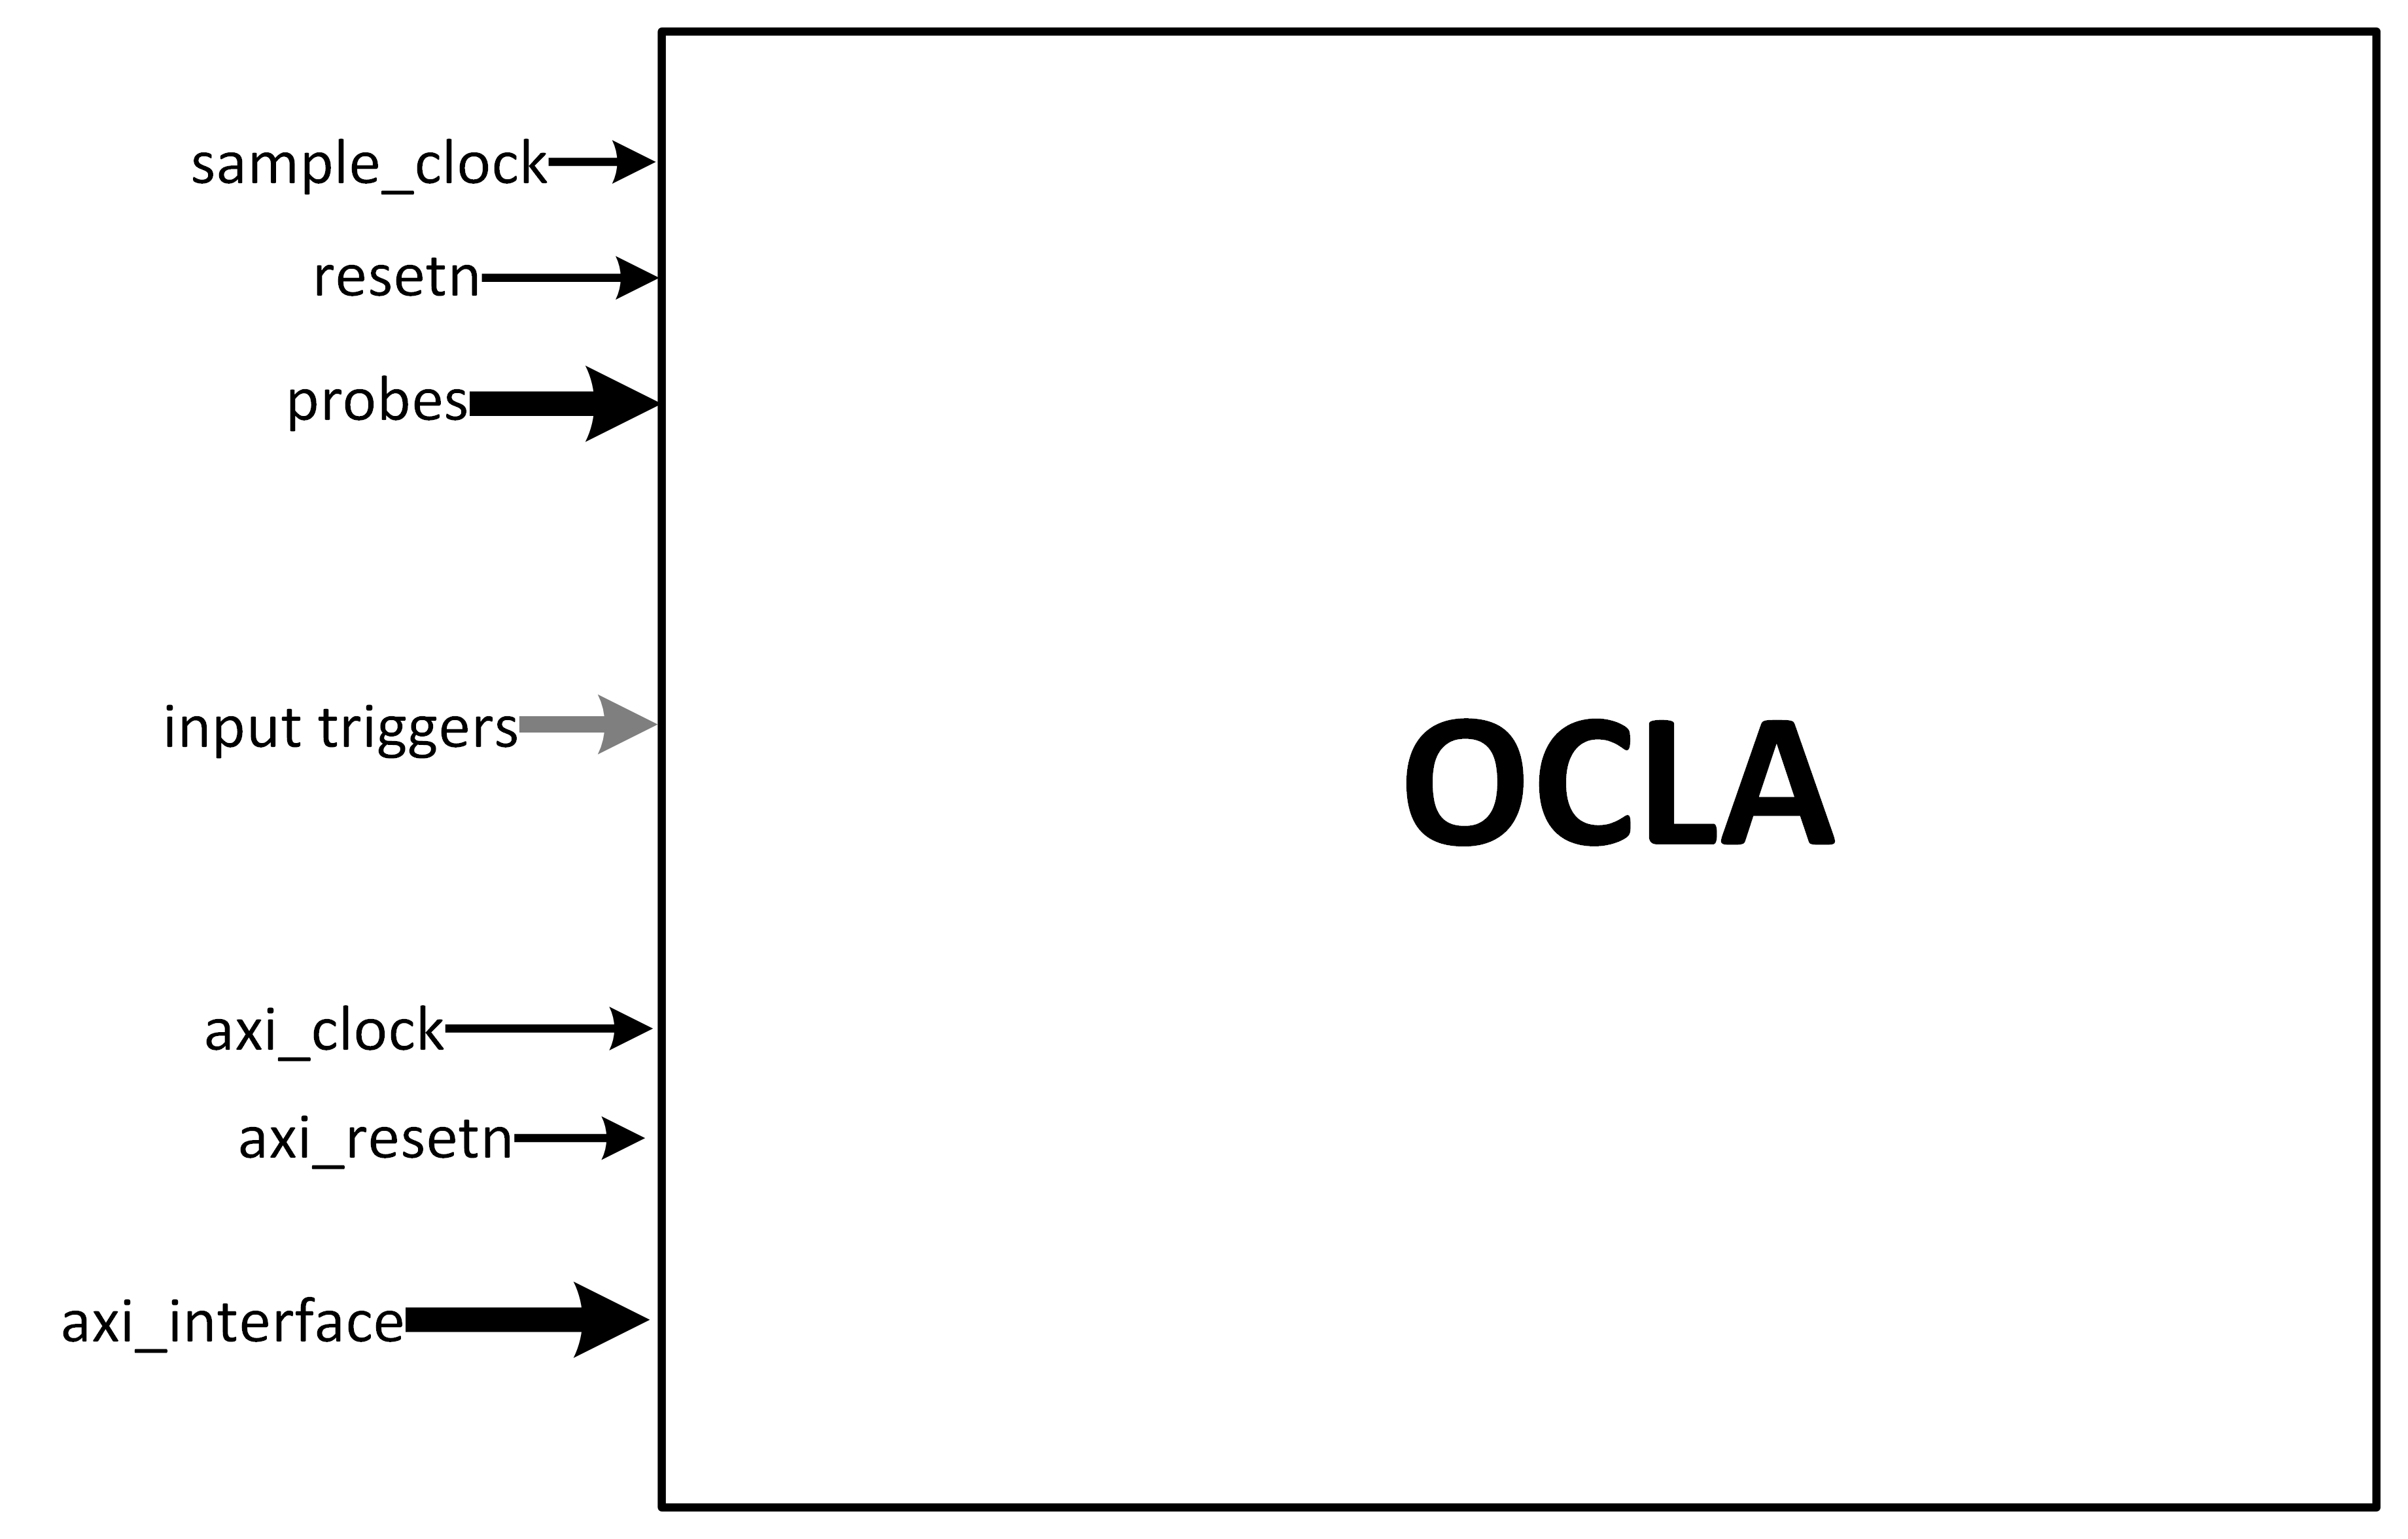
\includegraphics[width=.5\linewidth]{ocla_wrpr}
	\caption{OCLA Top}
	\label{fig:ocla_wrpr}
\end{figure}
% \lipsum
\newpage
\subsection*{\fontsize{14}{16}\selectfont Licensing}
\addcontentsline{toc}{subsection}{Licensing}
% COPYRIGHT TEXT:\\
% \line(1,0){100}\\

Copyright (c) 2022 RapidSilicon \\ \\
Permission is hereby granted, free of charge, to any person obtaining a copy of
this software and associated documentation files (the "Software"), to deal in
the Software without restriction, including without limitation the rights to
use, copy, modify, merge, publish, distribute, sublicense, and/or sell copies of
the Software, and to permit persons to whom the Software is furnished to do so,
subject to the following conditions: The above copyright notice and this
permission notice shall be included in all copies or substantial portions of the
Software.
\\ \\
THE SOFTWARE IS PROVIDED "AS IS", WITHOUT WARRANTY OF ANY KIND, EXPRESS OR
IMPLIED, INCLUDING BUT NOT LIMITED TO THE WARRANTIES OF MERCHANTABILITY, FITNESS
FOR A PARTICULAR PURPOSE AND NONINFRINGEMENT. IN NO EVENT SHALL THE AUTHORS OR
COPYRIGHT HOLDERS BE LIABLE FOR ANY CLAIM, DAMAGES OR OTHER LIABILITY, WHETHER
IN AN ACTION OF CONTRACT, TORT OR OTHERWISE, ARISING FROM, OUT OF OR IN
CONNECTION WITH THE SOFTWARE OR THE USE OR OTHER DEALINGS IN THE SOFTWARE.
\par\noindent\rule{\textwidth}{0.4pt}
\newpage
\section*{\hfill IP Specification}
\addcontentsline{toc}{section}{IP Specification}

\subsection*{\fontsize{14}{16}\selectfont Overview}
\addcontentsline{toc}{subsection}{Overview}

\paragraph{} The figure \ref{fig:ocla1} shows the internal block diagram of OCLA. It is a modular design consisting various modules like OCLA AXI-lite Slave interface, Trigger Control Unit, Sampler Buffer, OCLA Contoller and OCLA On-Chip Trace Memory modules.
\\ It is a multi-clock design and it has a sampling clock as well as the AXI bus clock. The sampling clock is the same clock as the clock of the System/Design under test (S/DUT).\\ Data is sampled on the rising edge of this sample clock based on the configured sampling mode of the OCLA. The OCLA is configured through the AXI interface on the rising edge of the AXI bus clock. The sampled data can be read via the AXI interface running on rising edge of the AXI clock. 
\\The modules that controls the sampling operation of the OCLA operate on the sampling clock. For example the sampler buffer and the OCLA controler operates on sampling clock.
On the other hand the AXI Slave and the Stream Out Buffer is modules operate on the AXI clock and these modules are used to configure or read the aquired data from the trace memory.\\
The On-Chip trace memory controller is a circular buffer based on a modified asynchronous FIFO that handles clock domain crossing of the trace memory data and configuration data .    

\begin{figure}[h]\centering % Using \begin{figure*} makes the figure take up the entire width of the page
	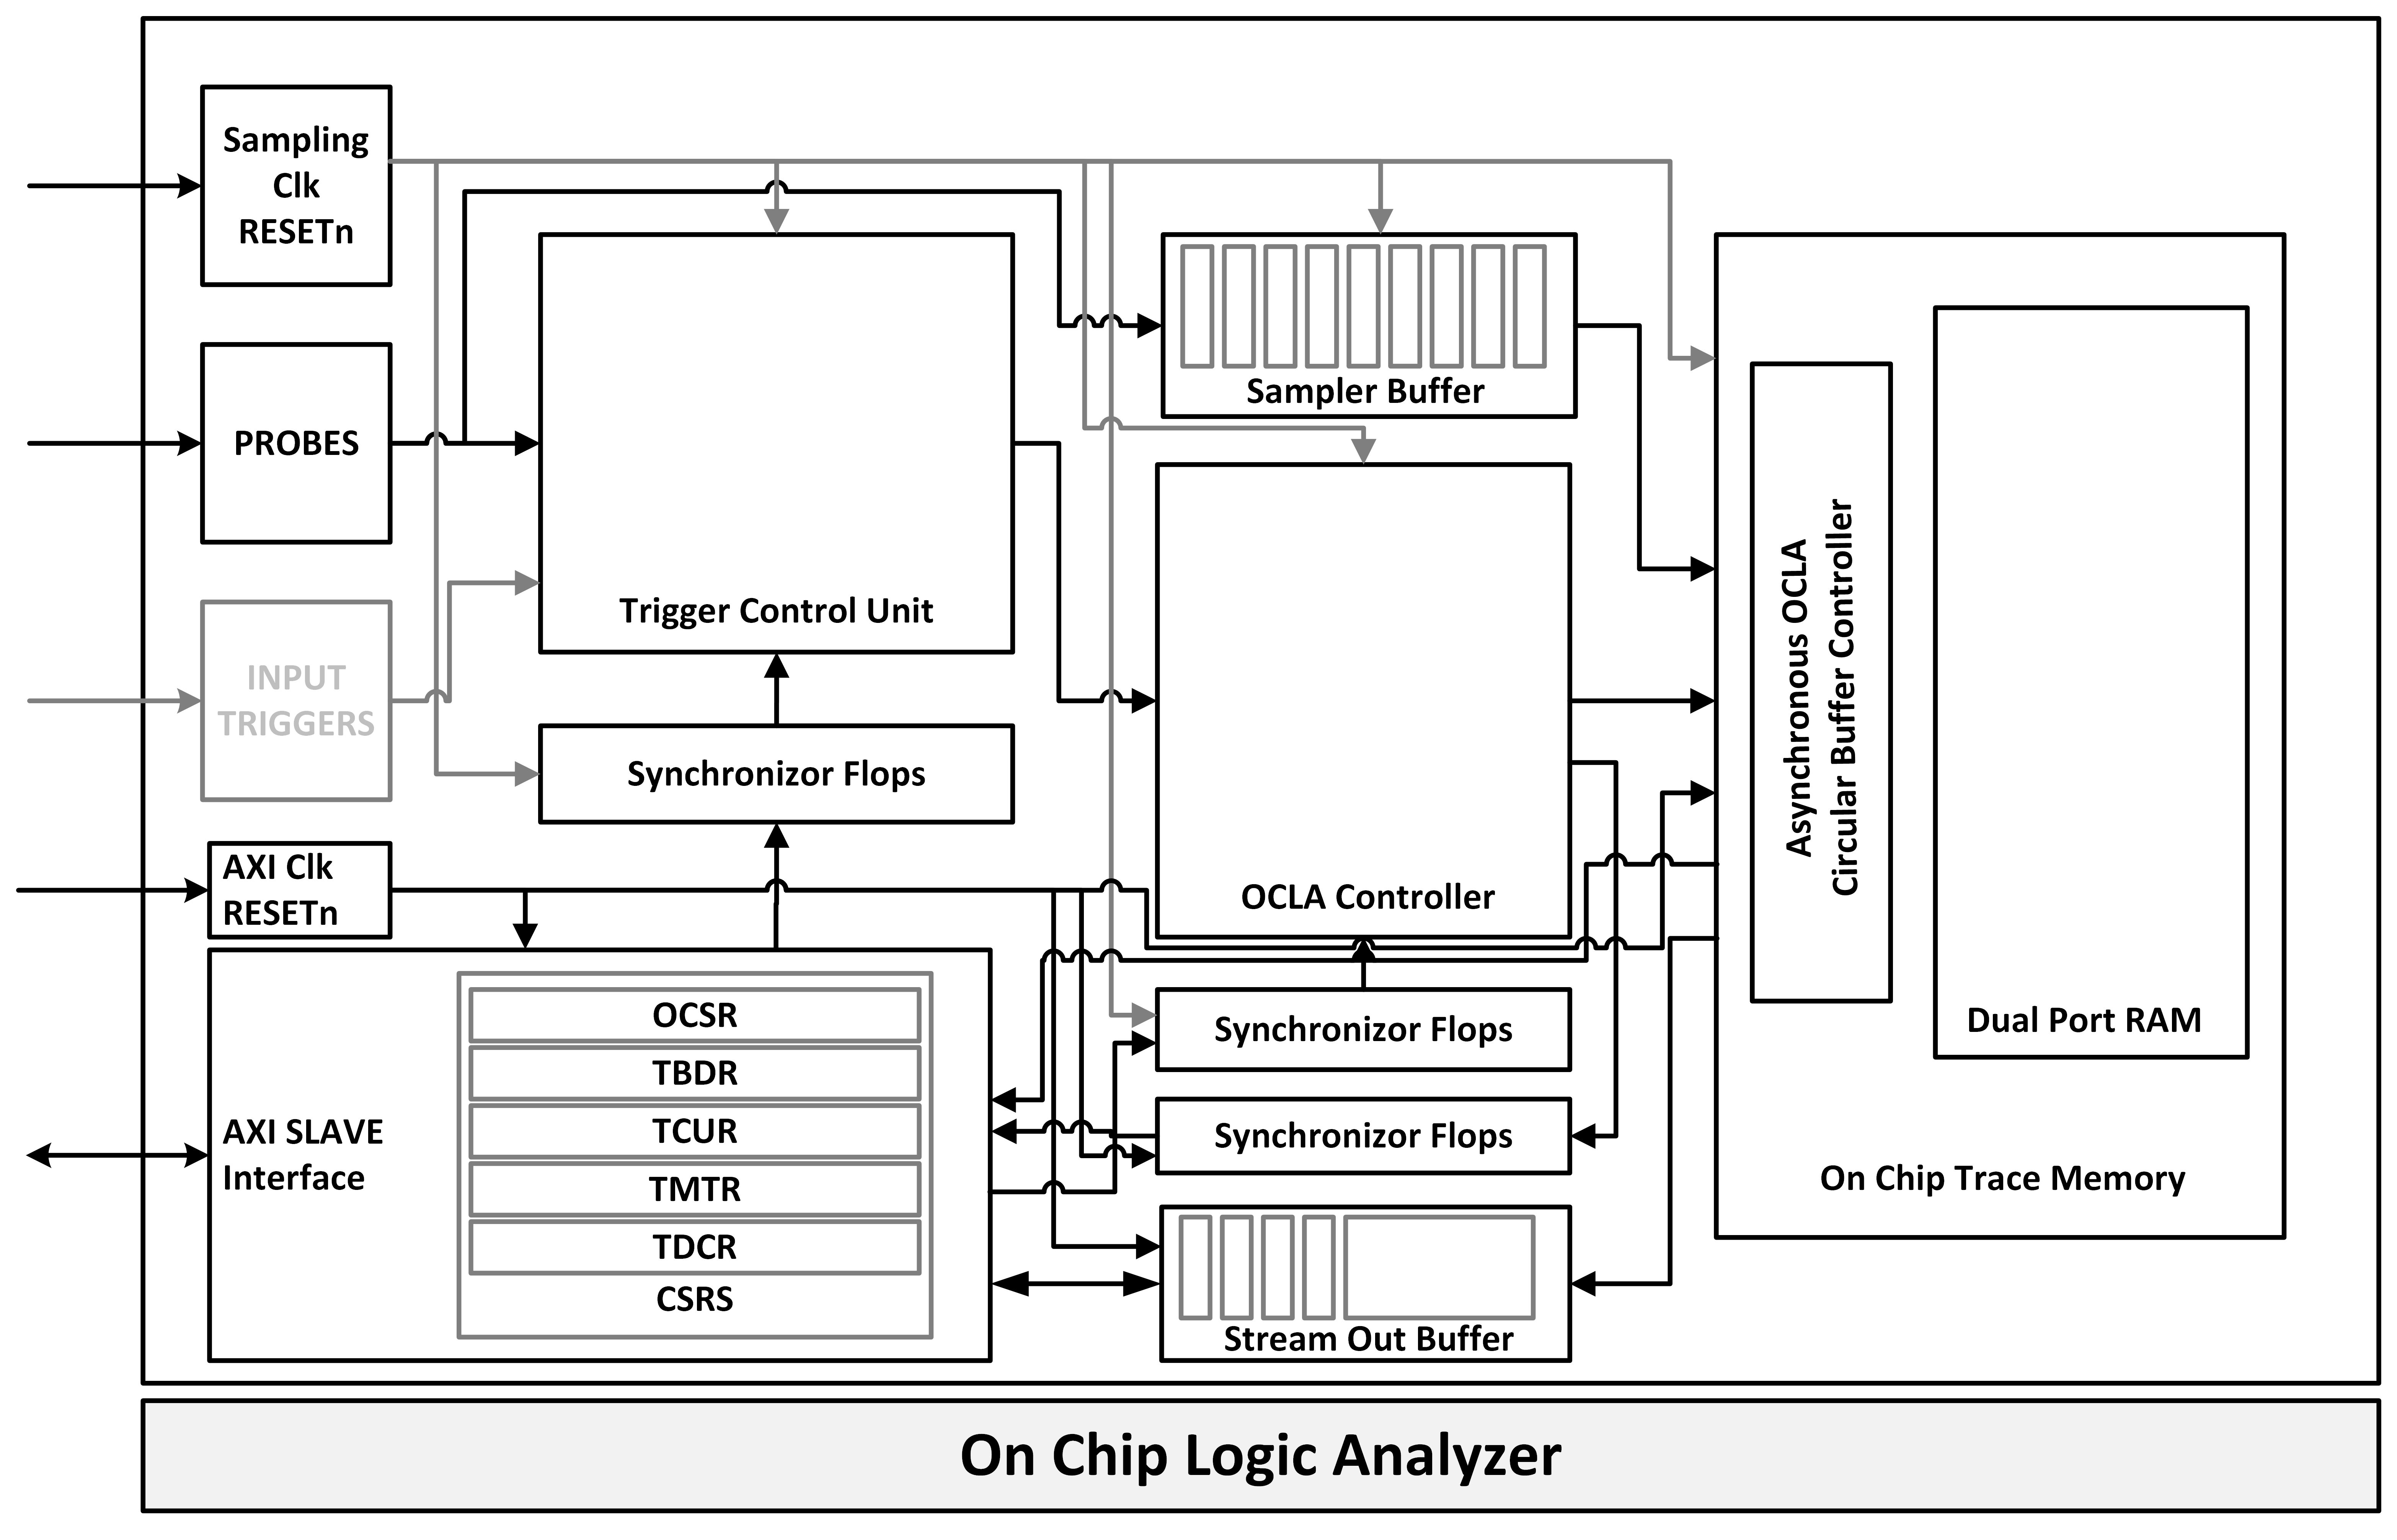
\includegraphics[width=\linewidth]{ocla1}
	\caption{Top Module}
	\label{fig:ocla1}
\end{figure}


\subsection*{\fontsize{14}{16}\selectfont Trigger}
\paragraph{}Triggers can be defined to configure the OCLA for capturing probe data samples. A probe input signal or a trigger input signal can be set as a trigger signal. A variety of trigger conditions can be configured on the trigger signal. Data sampling begins when all of the trigger conditions in the active trigger pattern are satisfied. A Trigger Position setting (Trigger mode) allows the user to specify the amount of data captured by the OCLA that should be acquired before the trigger and the amount that should be acquired after the trigger. Acquired data is placed in a circular buffer.
\paragraph{}OCLA supports simple and advance trigger options.
\begin{itemize}[noitemsep]
	\item In simple trigger option configuration the trigger condition can be applied on only a single probe channel.
	\item In advance triifer option configuration the trigger condition can be applied on two probe channels with boolean comparison applicable on their trigger conditions. 
\end{itemize}
\subsection*{\fontsize{14}{16}\selectfont Trigger Conditions}
\paragraph{}Multiple options for trigger conditions are available for probe and input triggers signals. Following lists the trigger conditions:
\begin{longtable}{|l|l|}
	\hline
	\textbf{Trigger Condition} & \textbf{Description}                                                                                                \\ \hline
	\endfirsthead
	%
	\endhead
	%
	Don’t Care                 & Default trigger condition. The channel is not \\ & used to determine the trigger event.                                  \\ \hline
	Low level                  & OCLA triggers when the probe channel is low.                                                                              \\ \hline
	High level                 & OCLA triggers when the probe channel is high.                                                                             \\ \hline
	Falling Edge               & OCLA triggers on the falling edge the probe channel.                                                                          \\ \hline
	Rising Egde                & OCLA triggers on the falling edge the probe channel.                                                                           \\ \hline
	Either Edge                & OCLA triggers on either edge of the probe channel.                                                                \\ \hline
	Value Comparison           & OCLA triggers when the value of a probe channel is \\ & equal /less than / greator than some user specified value.       \\ \hline

	Boolean Trigger equations  & \begin{tabular}[c]{@{}l@{}}Advance Trigger Conditions AND, OR, \\  \textless{}, \textgreater{}, == etc\end{tabular} \\ \hline
	\caption{Trigger Conditions}
	\label{tab:Trigger-Condition}                                                                                                                    \\
\end{longtable}
\subsection*{\fontsize{14}{16}\selectfont Trigger Modes}
\paragraph{} The common trigger modes are post trig, pre trig, center and countinous.
\begin{itemize}[noitemsep]
	\item In \textbf{pre triggered} the
	      stored data set will consist of data sampled after the trigger.
	\item \textbf{Post triggered} is the opposite and in
	      this mode the logic analyzer stops the sampling immediately when the trigger is raised
	      thus only storing data from before the triggering event.
	\item \textbf{Center triggered} is a combination putting the
	      triggering event in the middle of the sampled data set
	\item \textbf{Continous trigger} mode continounsly samples data.
\end{itemize}

\subsection*{ Fix number of samples}
\paragraph{} OCLA can be configured on run time to sample a specfic number of probe samples other than the trace memory depth.
\subsection*{\fontsize{14}{16}\selectfont Standards}
\addcontentsline{toc}{subsection}{Standards}
The AXI4-Lite Slave interface is compliant with the AMBA® AXI Protocol
Specification.
\par\noindent\rule{\textwidth}{0.4pt}
  % \lipsum
\newpage
  \subsection*{\fontsize{14}{16}\selectfont IP Support Details}
  \addcontentsline{toc}{subsection}{IP Support Details}


  \begin{table}[h!]
	\resizebox{\columnwidth}{!}{%
	\begin{tabular}{|ll|lllll|lll|}
	\hline
	\multicolumn{2}{|c|}{\textbf{Compliance}} &
	  \multicolumn{5}{c|}{\textbf{IP Resources}} &
	  \multicolumn{3}{c|}{\textbf{Tool Flow}} \\ \hline
	\multicolumn{1}{|l|}{\textbf{Device}} &
	  \textbf{Interface} &
	  \multicolumn{1}{l|}{\textbf{Source Files}} &
	  \multicolumn{1}{l|}{\textbf{Constraint File}} &
	  \multicolumn{1}{l|}{\textbf{Testbench}} &
	  \multicolumn{1}{l|}{\textbf{Simulation Model}} &
	  \textbf{Software Driver} &
	  \multicolumn{1}{l|}{\textbf{Analyze and Elaboration}} &
	  \multicolumn{1}{l|}{\textbf{Simulation}} &
	  \textbf{Synthesis} \\ \hline
	\multicolumn{1}{|l|}{GEMINI} &
	  AXI4-lite &
	  \multicolumn{1}{l|}{Systemverilog} &
	  \multicolumn{1}{l|}{SDC} &
	  \multicolumn{1}{l|}{Systemverilog} &
	  \multicolumn{1}{l|}{-} &
	  - &
	  \multicolumn{1}{l|}{Raptor} &
	  \multicolumn{1}{l|}{Raptor} &
	  Raptor \\ \hline
	\end{tabular}%
	}
	\end{table}

\subsection*{\fontsize{14}{16}\selectfont Resource Utilization}
\addcontentsline{toc}{subsection}{Resource Utilization}


\noindent\begin{minipage}{\linewidth}
	\centering
	\resizebox{\linewidth}{!}{%
	\begin{tabular}{|>{\hspace{0pt}}m{0.179\linewidth}|>{\hspace{0pt}}m{0.296\linewidth}|>{\hspace{0pt}}m{0.187\linewidth}|>{\hspace{0pt}}m{0.156\linewidth}|>{\hspace{0pt}}m{0.119\linewidth}|} 
	\hline
	\multicolumn{1}{|>{\centering\hspace{0pt}}m{0.179\linewidth}|}{\textbf{Tool}} & \multicolumn{4}{>{\hspace{0pt}}m{0.758\linewidth}|}{Raptor Design Suite} \\ 
	\hline
	\multicolumn{1}{|>{\centering\hspace{0pt}}m{0.179\linewidth}|}{\textbf{FPGA Device}} & \multicolumn{4}{>{\hspace{0pt}}m{0.758\linewidth}|}{GEMINI} \\ 
	\hline
	\multicolumn{3}{|>{\centering\hspace{0pt}}m{0.661\linewidth}|}{\textbf{Configuration}} & \multicolumn{2}{>{\centering\arraybackslash\hspace{0pt}}m{0.275\linewidth}|}{\textbf{Resource Utilization}} \\ 
	\hline
	\multirow{6}{0.179\linewidth}{\hspace{0pt}\begin{tabular}[c]{@{}l@{}}Minimum \\Resource\end{tabular}} & \textbf{Options} & \textbf{Configuration} & \textbf{Resources} & \textbf{Utilized} \\ 
	\cline{2-5}
	 & Number of Probe & 1 & LUT & 263 \\ 
	\cline{2-5}
	 & Trace Memory Depth & 32 & DFFR & 90 \\ 
	\cline{2-5}
	 & Advance Trigger Mode & OFF & DFFRE & 148 \\ 
	\cline{2-5}
	 & Value Compare Feature & OFF & BRAM & 1 \\ 
	\cline{2-5}
	 & Input Triggers & 0 & DSP & 0 \\ 
	\hline
	\multirow{6}{0.179\linewidth}{\hspace{0pt}\begin{tabular}[c]{@{}l@{}}Maximum \\Resource\end{tabular}} & \textbf{Options} & \textbf{Configuration} & \textbf{Resources} & \textbf{Utilized} \\ 
	\cline{2-5}
	 & Number of Probe & 1024 & LUT & 1068 \\ 
	\cline{2-5}
	 & Trace Memory Depth & 1024 & DFFR & 4260 \\ 
	\cline{2-5}
	 & Advance Trigger Mode & ON & DFFRE & 1206 \\ 
	\cline{2-5}
	 & Value Compare Feature & ON & BRAM & 29 \\ 
	\cline{2-5}
	 & Input Triggers & 32 & DSP & 0 \\
	\hline
	\end{tabular}
	}
	\end{minipage}
  % \lipsum
  \newpage
\subsection*{\fontsize{14}{16}\selectfont Ports}
\addcontentsline{toc}{subsection}{Port List}

\paragraph{} Table \ref{tab:ocla-intr} lists the top interface ports of the OCLA.

% \usepackage{array}
% \usepackage{longtable}
% \usepackage{colortbl}


  
\begin{longtable}{|>{\hspace{0pt}}m{0.292\linewidth}|>{\centering\hspace{0pt}}m{0.056\linewidth}|>{\hspace{0pt}}m{0.585\linewidth}|} 
\hline
 \multicolumn{1}{|>{\centering\hspace{0pt}}m{0.292\linewidth}|}{\textbf{  {Signal Name}}} & \textbf{  {I/O}} & \multicolumn{1}{>{\centering\arraybackslash\hspace{0pt}}m{0.585\linewidth}|}{\textbf{  {Description}}} \endfirsthead
 \hline
 \multicolumn{3}{|>{\hspace{0pt}}m{0.932\linewidth}|}{\textbf{Sampling Clock and Reset }} \\ 
\hline
i\_sample\_clk & I & Clock to Sample the Probe Data.\par{}It must be same as the Design under test \\ 
\hline
i\_rstn & I & Reset port of OCLA and it must be same\par{}~as design under test \\ 
\hline
\multicolumn{3}{|>{\hspace{0pt}}m{0.932\linewidth}|}{\textbf{AXI Clock and Reset }} \\ 
\hline
i\_S\_AXI\_ACLK & I & AXI4-Lite Clock \\ 
\hline
i\_S\_AXI\_ARESETN & I & AXI4-Lite RESET \\ 
\hline
\multicolumn{3}{|>{\hspace{0pt}}m{0.932\linewidth}|}{\textbf{AXI WRITE ADDRESS CHANNEL }} \\ 
\hline
s\_axil\_awvalid & I & AXI4-Lite Write address valid \\ 
\hline
s\_axil\_awready & O & AXI4-Lite Write address ready \\ 
\hline
s\_axil\_awaddr & I & AXI4-Lite Write address \\ 
\hline
s\_axil\_awprot & I & AXI4-Lite Protection type \\ 
\hline
\multicolumn{3}{|>{\hspace{0pt}}m{0.932\linewidth}|}{\textbf{AXI WRITE DATA CHANNEL }} \\ 
\hline
s\_axil\_wvalid & I & AXI4-Lite Write valid \\ 
\hline
s\_axil\_wready & O & AXI4-Lite Write ready. \\ 
\hline
s\_axil\_wdata & I & AXI4-Lite Write data \\ 
\hline
s\_axil\_wstrb & I & AXI4-Lite Write strobes \\ 
\hline
\multicolumn{3}{|>{\hspace{0pt}}m{0.932\linewidth}|}{\textbf{AXI WRITE RESPONSE CHANNEL }} \\ 
\hline
s\_axil\_bvalid & O & AXI4-Lite~ Write response valid \\ 
\hline
s\_axil\_bready & I & AXI4-Lite Response ready \\ 
\hline
s\_axil\_bresp & O & AXI4-Lite Write response \\ 
\hline
\multicolumn{3}{|>{\hspace{0pt}}m{0.932\linewidth}|}{\textbf{AXI READ ADDRESS CHANNEL }} \\ 
\hline
s\_axil\_arvalid & I & AXI4-Lite Read address valid \\ 
\hline
s\_axil\_arready & O & AXI4-Lite Read address ready \\ 
\hline
s\_axil\_araddr & I & AXI4-Lite Read address \\ 
\hline
s\_axil\_arprot & I & AXI4-Lite Protection type \\ 
\hline
\multicolumn{3}{|>{\hspace{0pt}}m{0.932\linewidth}|}{\textbf{AXI READ DATA CHANNEL }} \\ 
\hline
s\_axil\_rvalid & I & AXI4-Lite Read valid \\ 
\hline
s\_axil\_rready & O & AXI4-Lite Read ready \\ 
\hline
s\_axil\_rresp & I & AXI4-Lite Read data \\ 
\cline{1-2}
s\_axil\_rdata & O & AXI4-Lite Read response \\ 
\hline
\multicolumn{3}{|>{\hspace{0pt}}m{0.932\linewidth}|}{\textbf{OCLA PORTS }} \\ 
\hline
i\_probes & I & OCLA Probes port~ \\ 
\hline
i\_trigger\_input & I & OCLA Trigger input port. It is\par{}~an optional port \\
\hline
\end{longtable}
\captionsetup{labelformat=empty}
\captionof{table}{OCLA Interface}
\label{tab:ocla-intr} 
\arrayrulecolor{black}

	
\subsection*{\fontsize{14}{16}\selectfont Parameters}
\addcontentsline{toc}{subsection}{Parameters}

\paragraph{} Table \ref{tab:config-param} lists the parameters of the OCLA.
% Please add the following required packages to your document preamble:
% \usepackage{longtable}
% Note: It may be necessary to compile the document several times to get a multi-page table to line up properly

\noindent\begin{minipage}{\linewidth}
	\centering
	  
	\resizebox{\linewidth}{!}{%
	\begin{tabular}{|>{\centering\hspace{0pt}}m{0.188\linewidth}|>{\centering\hspace{0pt}}m{0.16\linewidth}|>{\centering\hspace{0pt}}m{0.096\linewidth}|>{\hspace{0pt}}m{0.492\linewidth}|} 
	\hline
	    {\textbf{Parameter}~} &   {\textbf{Values~~}} &   {\textbf{Default Value~}} & \multicolumn{1}{>{\centering\arraybackslash\hspace{0pt}}m{0.492\linewidth}|}{\textbf{  {Description~}}} \\ 
	\hline
	NUMBER OF PROBES & 1-1024~ & 1~ & Number of OCLA probe ports. \\ 
	\hline
	MEMORY DEPTH & 32, 64, 128, 256, 512,1024 & 32 & Probe storage buffer depth. This number\par{}represents the maximum number of samples that can be stored at run time for each probe input. \\ 
	\hline
	NUMBER OF INPUT TRIGGERS & 1-31~ & 1 & Number of trigger input ports. \\ 
	\hline
	PROBE WIDTH & 1-31~ & 1 & Probe width in case of value compare mode \\
	\hline
	\end{tabular}
	}
	\arrayrulecolor{black}
	\captionsetup{labelformat=empty}
	\captionof{table}{Parameters}
	\label{tab:config-param} 
	\end{minipage}


	% \usepackage{array}
% \usepackage{graphicx}
% \usepackage{hhline}
% \usepackage{colortbl}
\subsection*{\fontsize{14}{16}\selectfont Optional Macros }
\addcontentsline{toc}{subsection}{Optional Macros}
\paragraph{} Table \ref{tab:op-macro} lists the Macors of the OCLA.



\noindent\begin{minipage}{\linewidth}
	\centering
	\resizebox{\linewidth}{!}{%
	\begin{tabular}{|>{\hspace{0pt}}m{0.3\linewidth}|>{\hspace{0pt}}m{0.221\linewidth}|>{\hspace{0pt}}m{0.417\linewidth}|} 
	\hline
	\textbf{ Feature} & \textbf{ Macro} & \textbf{ Description} \\ 
	\hline
	Value Compare Feature & value\_compare & To enable Value Compare feature \\ 
	\hline
	Advance Trigger Mode & advance\_trigger & To enable Advance Trigger Mode \\ 
	\hline
	Enable Trigger Inputs & trigger\_inputs\_en & To enable Trigger inputs \\
	\hline
	\end{tabular}
	}\arrayrulecolor{black}
	\captionsetup{labelformat=empty}
	\captionof{table}{Parameters}
	\label{tab:op-macro} 
	\end{minipage}

%%%%%%%%%%%%%%%%%%%%%%%%%%%%%%%%%%%%%%%%%%%%%%%%%%%%%%%%%%%%%%%%%%%%%%%%%%%%%%%%%%%%%%%%%%%%%%%%%%%%%%%%
%    Register space and CSRs bitfield descriptions
%    Commented in user IP guide document. 
%
%
%%%%%%%%%%%%%%%%%%%%%%%%%%%%%%%%%%%%%%%%%%%%%%%%%%%%%%%%%%%%%%%%%%%%%%%%%%%%%%%%%%%%%%%%%%%%%%%%%%%%%%%%


% \subsection*{\fontsize{14}{16}\selectfont Registers Address Space}
% \addcontentsline{toc}{subsection}{Registers Address Space}

% \paragraph{} Table \ref{tab:config-reg} lists the configuration registers of the OCLA.
% % Please add the following required packages to your document preamble:
% % \usepackage{longtable}
% % Note: It may be necessary to compile the document several times to get a multi-page table to line up properly
% % Please add the following required packages to your document preamble:
% % \usepackage{longtable}
% % Note: It may be necessary to compile the document several times to get a multi-page table to line up properly
% \footnotesize



% \noindent\begin{minipage}{\linewidth}
% 	\centering
	  
% 	\resizebox{\linewidth}{!}{%
% 	\begin{tabular}{|>{\hspace{0pt}}m{0.194\linewidth}|>{\centering\hspace{0pt}}m{0.117\linewidth}|>{\centering\hspace{0pt}}m{0.058\linewidth}|>{\centering\hspace{0pt}}m{0.073\linewidth}|>{\centering\hspace{0pt}}m{0.096\linewidth}|>{\centering\hspace{0pt}}m{0.135\linewidth}|>{\hspace{0pt}}m{0.258\linewidth}|}
% 	% \multicolumn{7}{>{\centering\arraybackslash\hspace{0pt}}m{0.931\linewidth}}{\textbf{Configuration Registers}} \\ 
% 	\hline
% 	  \multicolumn{1}{|>{\centering\hspace{0pt}}m{0.194\linewidth}|}{\textbf{  {Name~}}} & \textbf{  {Register ID~}} & \textbf{  {Bits}}~ & \textbf{  {Type}}~~ & \textbf{  {Off sets~~}} & \textbf{  {Default Value~}} & \multicolumn{1}{>{\centering\arraybackslash\hspace{0pt}}m{0.258\linewidth}|}{\textbf{  {Description~}}} \\ 
% 	\hline
% 	OCLA Status \par{}Register~ & OCSR~ & 32~ & RO~ & 0x00~ & 0xC0000000 & Bitfields of this OCSR contains\par{}~configuration status of OCLA \\ 
% 	\hline
% 	Trace Buffer Data\par{}~Register~ & TBDR~ & 32~ & RO~ & 0x04~ & 0x00000000 & TBDR can be read to \par{}stream the whole acquisition \par{}data to some output interface \\ 
% 	\hline
% 	Trigger Control\par{}~Register~ & TCUR~ & 32~ & RW~ & 0x08~ & 0x00000000 & ~TCUR is used to control \par{}the trigger control unit \\ 
% 	\hline
% 	Trigger Mode Type~ \par{}Register~ & TMTR~ & 32~ & RW~ & 0x0C~ & 0x00000000 & TMCR is used configure\par{}~trigger Modes~ \\ 
% 	\hline
% 	Trigger Data Compare \par{}Register & TDCR & 32~ & RW~ & 0x10~ & 0x00000000 & ~Trigger Data to compare with\par{}~the probe port \\
% 	\hline
% 	\end{tabular}
% 	}
% 	\captionsetup{labelformat=empty}
% 	\captionof{table}{Configuration Registers}
% 	\arrayrulecolor{black}
% 	\label{tab:config-reg} 
% 	\end{minipage}


% 	\newpage
% %
% \subsection*{\fontsize{14}{16}\selectfont CSRs Description}
% \addcontentsline{toc}{subsection}{CSRs Description}

% \paragraph{OCLA Status Register}


% \normalsize
% \begin{itemize}[noitemsep]
% 	\item [] OCLA Status Register is a read-only register. This register contains the OCLA ID and samling status which are described in the following table.
% \end{itemize}


% \noindent\begin{minipage}{\linewidth}
% 	\centering
% 	\resizebox{\linewidth}{!}{%
% 	\begin{tabular}{|>{\hspace{0pt}}m{0.131\linewidth}|>{\hspace{0pt}}m{0.225\linewidth}|>{\hspace{0pt}}m{0.087\linewidth}|>{\hspace{0pt}}m{0.131\linewidth}|>{\hspace{0pt}}m{0.363\linewidth}|} 
% 	\hline
% 	\textbf{ Bits} & \textbf{ Description} & \textbf{ Bitfield} & \textbf{ Values} & \textbf{ Configuration} \\ 
% 	\hline
% 	\multirow{2}{0.131\linewidth}{\hspace{0pt}DA} & \multirow{2}{0.225\linewidth}{\hspace{0pt}\begin{tabular}[c]{@{}l@{}}Indicates that sampled \\data is available in the \\OCLA memory\\\end{tabular}} & \multirow{2}{0.087\linewidth}{\hspace{0pt}0]} & 0 & Sampling is not done yet \\ 
% 	\cline{4-5}
	
% 	 &  &  & 1 & Sampling is done and \par{}sampled data is available for reading~ \\ 
% 	 &  &  & 1 &\\ 
% 	\hline
% 	RESERVED & RESERVED & {[}29:1] & RESERVED & RESERVED \\ 
% 	\hline
% 	ID & OCLA ID & {[}31:30] & 11 & These two bits represents the OCLA \par{}ID. For OCLA these bits\par{}are always high \\
% 	\hline
% 	\end{tabular}
% 	}
% 	\end{minipage}

  





% \paragraph{Trace Buffer data Register}
% %
% % Please add the following required packages to your document preamble:
% % \usepackage{booktabs}
% % \usepackage{graphicx}
% \begin{itemize}[noitemsep]
% 	\item [] Trace Buffer data Register is used to streamed off the acquired data via the AXI-Slave interface from the internal trace memory of the OCLA

% \end{itemize}
% %


% \noindent\begin{minipage}{\linewidth}
% 	\centering
% 	\captionsetup{labelformat=empty}
% 	\captionof{table}{OCSR Register}\resizebox{\linewidth}{!}{%
% 	\begin{tabular}{|>{\hspace{0pt}}m{0.026\linewidth}>{\hspace{0pt}}m{0.026\linewidth}>{\hspace{0pt}}m{0.026\linewidth}>{\hspace{0pt}}m{0.026\linewidth}>{\hspace{0pt}}m{0.026\linewidth}>{\hspace{0pt}}m{0.026\linewidth}>{\hspace{0pt}}m{0.026\linewidth}>{\hspace{0pt}}m{0.026\linewidth}>{\hspace{0pt}}m{0.026\linewidth}>{\hspace{0pt}}m{0.026\linewidth}>{\hspace{0pt}}m{0.026\linewidth}>{\hspace{0pt}}m{0.026\linewidth}>{\hspace{0pt}}m{0.026\linewidth}>{\hspace{0pt}}m{0.026\linewidth}>{\hspace{0pt}}m{0.026\linewidth}>{\hspace{0pt}}m{0.026\linewidth}>{\hspace{0pt}}m{0.026\linewidth}>{\hspace{0pt}}m{0.026\linewidth}>{\hspace{0pt}}m{0.026\linewidth}>{\hspace{0pt}}m{0.026\linewidth}>{\hspace{0pt}}m{0.026\linewidth}>{\hspace{0pt}}m{0.026\linewidth}>{\hspace{0pt}}m{0.026\linewidth}>{\hspace{0pt}}m{0.026\linewidth}>{\hspace{0pt}}m{0.026\linewidth}>{\hspace{0pt}}m{0.026\linewidth}>{\hspace{0pt}}m{0.026\linewidth}>{\hspace{0pt}}m{0.026\linewidth}>{\hspace{0pt}}m{0.026\linewidth}>{\hspace{0pt}}m{0.026\linewidth}>{\hspace{0pt}}m{0.026\linewidth}>{\hspace{0pt}}m{0.026\linewidth}|} 
% 	\hline
% 	31 & 30 & 29 & 28 & 27 & 26 & 25 & 24 & 23 & 22 & 21 & 20 & 19 & 18 & 17 & 16 & 15 & 14 & 13 & 12 & 11 & 10 & 9 & 8 & 7 & 6 & 5 & 4 & 3 & 2 & 1 & 0 \\ 
% 	\hline
% 	\multicolumn{32}{|>{\hspace{0pt}}m{0.832\linewidth}|}{\textbf{Trace Buffer Data}} \\
% 	\hline
% 	\end{tabular}
% 	}
% 	\end{minipage}

% 	\newpage

% 	\paragraph{Trigger Mode Type Register}
% 	\begin{itemize}[noitemsep]
% 		\item [] Trigger Mode Type Register can be used to configure the trigger samples modes of the OCLA. The following table describes the bitfields of this register for different modes of configuration of the OCLA.
% 	\end{itemize}
	
	  

% 	\noindent\begin{minipage}{\linewidth}
% 		\centering
% 		\captionsetup{labelformat=empty}
% 		\captionof{table}{TMTR Register}\resizebox{\linewidth}{!}{%
% 		\begin{tabular}{|>{\hspace{0pt}}m{0.102\linewidth}|>{\hspace{0pt}}m{0.319\linewidth}|>{\hspace{0pt}}m{0.087\linewidth}|>{\hspace{0pt}}m{0.079\linewidth}|>{\hspace{0pt}}m{0.348\linewidth}|} 
% 		\hline
% 		\textbf{Bits} & \textbf{Description} & \textbf{Bitfield} & \textbf{Values} & \textbf{Configuration} \\ 
% 		\hline
% 		\multirow{4}{0.102\linewidth}{\hspace{0pt}TM} & \multirow{4}{0.319\linewidth}{\hspace{0pt}Trigger Modes} & \multirow{4}{0.087\linewidth}{\hspace{0pt}{[}1:0]} & 0 0 & No trigger Continuous \\ 
% 		\cline{4-5}
% 		 &  &  & 0 1 & Pre Trigger \\ 
% 		\cline{4-5}
% 		 &  &  & 1 0 & Post trigger \\ 
% 		\cline{4-5}
% 		 &  &  & 1 1 & Center Trigger \\ 
% 		\hline
% 		ST & Start sampling & {[}2] & 1 & sampling enable \\ 
% 		\hline
% 		 &  &  & 0 & sampling disable \\ 
% 		\hline
% 		FNS & Fix number of samples option~ & {[}3] & 0 & disable sample fix number of samples \\ 
% 		\hline
% 		 &  &  & 1 & enable sample fix number of samples \\ 
% 		\hline
% 		NS & Number of samples to be sampled & {[}14:4] &  & user specified number\par{}~of samples \\ 
% 		\hline
% 		Reserved & Reserved & {[}31:15] &  & Reserved \\
% 		\hline
% 		\end{tabular}
% 		}
% 		\end{minipage}

% 	%
% 	\paragraph{Trigger Data Compare Register}
% 	\begin{itemize}[noitemsep]
% 		\item []Data For Comparison: User data to be compared with probe data for trigger event
% 	\end{itemize}


	

% \noindent\begin{minipage}{\linewidth}
% 	\centering
% 	\captionsetup{labelformat=empty}
% 	\captionof{table}{TMTR Register}\resizebox{\linewidth}{!}{%
% 	\begin{tabular}{|>{\hspace{0pt}}m{0.026\linewidth}>{\hspace{0pt}}m{0.026\linewidth}>{\hspace{0pt}}m{0.026\linewidth}>{\hspace{0pt}}m{0.026\linewidth}>{\hspace{0pt}}m{0.026\linewidth}>{\hspace{0pt}}m{0.026\linewidth}>{\hspace{0pt}}m{0.026\linewidth}>{\hspace{0pt}}m{0.026\linewidth}>{\hspace{0pt}}m{0.026\linewidth}>{\hspace{0pt}}m{0.026\linewidth}>{\hspace{0pt}}m{0.026\linewidth}>{\hspace{0pt}}m{0.026\linewidth}>{\hspace{0pt}}m{0.026\linewidth}>{\hspace{0pt}}m{0.026\linewidth}>{\hspace{0pt}}m{0.026\linewidth}>{\hspace{0pt}}m{0.026\linewidth}>{\hspace{0pt}}m{0.026\linewidth}>{\hspace{0pt}}m{0.026\linewidth}>{\hspace{0pt}}m{0.026\linewidth}>{\hspace{0pt}}m{0.026\linewidth}>{\hspace{0pt}}m{0.026\linewidth}>{\hspace{0pt}}m{0.026\linewidth}>{\hspace{0pt}}m{0.026\linewidth}>{\hspace{0pt}}m{0.026\linewidth}>{\hspace{0pt}}m{0.026\linewidth}>{\hspace{0pt}}m{0.026\linewidth}>{\hspace{0pt}}m{0.026\linewidth}>{\hspace{0pt}}m{0.026\linewidth}>{\hspace{0pt}}m{0.026\linewidth}>{\hspace{0pt}}m{0.026\linewidth}>{\hspace{0pt}}m{0.026\linewidth}>{\hspace{0pt}}m{0.026\linewidth}|} 
% 	\hline
% 	31 & 30 & 29 & 28 & 27 & 26 & 25 & 24 & 23 & 22 & 21 & 20 & 19 & 18 & 17 & 16 & 15 & 14 & 13 & 12 & 11 & 10 & 9 & 8 & 7 & 6 & 5 & 4 & 3 & 2 & 1 & 0 \\ 
% 	\hline
% 	\multicolumn{32}{|>{\hspace{0pt}}m{0.832\linewidth}|}{\textbf{Comparison For Data}} \\
% 	\hline
% 	\end{tabular}
% 	}
% 	\end{minipage}


% \newpage
% \paragraph[!]{Trigger Control Unit Register} 
% \begin{itemize}[noitemsep]

% \item [] Trigger Control Unit Register is used to configure the various trigger options. Following table shows the complete desrciption of the bitfields of this register.
% \end{itemize}

% \noindent\begin{minipage}{\linewidth}
% % \centering
% % \captionsetup{labelformat=empty}
% % \captionof{table}{}
% \resizebox{\linewidth}{!}{%
% \begin{tabular}{|>{\hspace{0pt}}m{0.026\linewidth}>{\hspace{0pt}}m{0.026\linewidth}>{\hspace{0pt}}m{0.026\linewidth}>{\hspace{0pt}}m{0.026\linewidth}>{\hspace{0pt}}m{0.026\linewidth}>{\hspace{0pt}}m{0.026\linewidth}>{\hspace{0pt}}m{0.026\linewidth}>{\hspace{0pt}}m{0.026\linewidth}>{\hspace{0pt}}m{0.026\linewidth}>{\hspace{0pt}}m{0.026\linewidth}>{\hspace{0pt}}m{0.026\linewidth}>{\hspace{0pt}}m{0.026\linewidth}>{\hspace{0pt}}m{0.026\linewidth}>{\hspace{0pt}}m{0.026\linewidth}>{\hspace{0pt}}m{0.026\linewidth}>{\hspace{0pt}}m{0.026\linewidth}>{\hspace{0pt}}m{0.026\linewidth}>{\hspace{0pt}}m{0.026\linewidth}>{\hspace{0pt}}m{0.026\linewidth}>{\hspace{0pt}}m{0.026\linewidth}>{\hspace{0pt}}m{0.026\linewidth}>{\hspace{0pt}}m{0.026\linewidth}>{\hspace{0pt}}m{0.026\linewidth}>{\hspace{0pt}}m{0.026\linewidth}>{\hspace{0pt}}m{0.026\linewidth}>{\hspace{0pt}}m{0.026\linewidth}>{\hspace{0pt}}m{0.026\linewidth}>{\hspace{0pt}}m{0.026\linewidth}>{\hspace{0pt}}m{0.026\linewidth}>{\hspace{0pt}}m{0.026\linewidth}>{\hspace{0pt}}m{0.026\linewidth}>{\hspace{0pt}}m{0.032\linewidth}|} 
% \hline
% 31 & 30 & 29 & 28 & 27 & 26 & 25 & 24 & 23 & 22 & 21 & 20 & 19 & 18 & 17 & 16 & 15 & 14 & 13 & 12 & 11 & 10 & 9 & 8 & 7 & 6 & 5 & 4 & 3 & 2 & 1 & 0 \\ 
% \hline
% \multicolumn{8}{|>{\hspace{0pt}}m{0.208\linewidth}|}{P2} & \multicolumn{7}{>{\hspace{0pt}}m{0.182\linewidth}|}{P1} & \multicolumn{2}{>{\hspace{0pt}}m{0.052\linewidth}|}{B} & \multicolumn{2}{>{\hspace{0pt}}m{0.052\linewidth}|}{V2} & L2 & \multicolumn{2}{>{\hspace{0pt}}m{0.052\linewidth}|}{E2} & \multicolumn{2}{>{\hspace{0pt}}m{0.052\linewidth}|}{C2} & \multicolumn{2}{>{\hspace{0pt}}m{0.052\linewidth}|}{V1} & L1 & \multicolumn{2}{>{\hspace{0pt}}m{0.052\linewidth}|}{E1} & \multicolumn{2}{>{\hspace{0pt}}m{0.052\linewidth}|}{C1} & O \\
% \hline
% \end{tabular}
% }
% \end{minipage}
  


% \noindent\begin{minipage}{\linewidth}
% 	\centering
% 	\captionsetup{labelformat=empty}
% 	\captionof{table}{TCUR Register}
% 	\resizebox{\linewidth}{!}{%
% 	\begin{tabular}{|>{\hspace{0pt}}m{0.056\linewidth}|>{\hspace{0pt}}m{0.448\linewidth}|>{\hspace{0pt}}m{0.09\linewidth}|>{\hspace{0pt}}m{0.16\linewidth}|>{\hspace{0pt}}m{0.171\linewidth}|} 
% 	\hline
% 	\textbf{Bits} & \textbf{Description} & \textbf{Bitfield} & \textbf{Values} & \textbf{Configuration} \\ 
% 	\hline
% 	\multirow{2}{0.056\linewidth}{\hspace{0pt}O} & \multirow{2}{0.448\linewidth}{\hspace{0pt}\begin{tabular}[c]{@{}l@{}}Trigger Option\\Simple Trigger: Only one signal can be \\selected as trigger signal\\Advance Trigger: Two signals can be \\selected as trigger signal and boolean\\~comparison can be applied on the \\two trigger events\end{tabular}} & \multirow{2}{0.09\linewidth}{\hspace{0pt}{[}0]} & 0 & Simple Trigger \\
% 	 &  &  &  &  \\
% 	 &  &  &  &  \\
% 	 &  &  &  &  \\ 
% 	\cline{4-5}
% 	 &  &  & 1 & Advance Trigger \\
% 	 &  &  &  &  \\
% 	 &  &  &  &  \\ 
% 	\hline
% 	\multirow{4}{0.056\linewidth}{\hspace{0pt}C1} & \multirow{4}{0.448\linewidth}{\hspace{0pt}\begin{tabular}[c]{@{}l@{}}Trigger Condition options\\for the first trigger signal\end{tabular}} & \multirow{4}{0.09\linewidth}{\hspace{0pt}{[}2:1]} & 0 0 & No trigger \\ 
% 	\cline{4-5}
% 	 &  &  & 0 1 & Edge Trigger \\ 
% 	\cline{4-5}
% 	 &  &  & 1 0 & Level Trigger \\ 
% 	\cline{4-5}
% 	 &  &  & 1 1 & Value Compare \\ 
% 	\hline
% 	\multirow{4}{0.056\linewidth}{\hspace{0pt}E1} & \multirow{4}{0.448\linewidth}{\hspace{0pt}\begin{tabular}[c]{@{}l@{}}Edge Trigger Type:\\Egde trigger options for the first trigger signal\end{tabular}} & \multirow{4}{0.09\linewidth}{\hspace{0pt}{[}4:3]} & 0 0 & No trigger \\ 
% 	\cline{4-5}
% 	 &  &  & 0 1 & Rising edge \\ 
% 	\cline{4-5}
% 	 &  &  & 1 0 & Falling edge \\ 
% 	\cline{4-5}
% 	 &  &  & 1 1 & Either edge \\ 
% 	\hline
% 	\multirow{2}{0.056\linewidth}{\hspace{0pt}L1} & \multirow{2}{0.448\linewidth}{\hspace{0pt}\begin{tabular}[c]{@{}l@{}}Level Trigger Type\\~Level trigger options for the first trigger signal\end{tabular}} & \multirow{2}{0.09\linewidth}{\hspace{0pt}{[}5]} & 0 & Low Level \\ 
% 	\cline{4-5}
% 	 &  &  & 1 & High Level \\ 
% 	\hline
% 	\multirow{4}{0.056\linewidth}{\hspace{0pt}V1} & \multirow{4}{0.448\linewidth}{\hspace{0pt}\begin{tabular}[c]{@{}l@{}}Value Compare Condition\\~trigger options for the first trigger signal\end{tabular}} & \multirow{4}{0.09\linewidth}{\hspace{0pt}{[}7:6]} & 0 0 & No trigger \\ 
% 	\cline{4-5}
% 	 &  &  & 0 1 & Equal to \\ 
% 	\cline{4-5}
% 	 &  &  & 1 0 & Less than \\ 
% 	\cline{4-5}
% 	 &  &  & 1 1 & Greater than \\ 
% 	\hline
% 	\multirow{4}{0.056\linewidth}{\hspace{0pt}C2} & \multirow{4}{0.448\linewidth}{\hspace{0pt}\begin{tabular}[c]{@{}l@{}}Trigger Condition\\options for the second trigger signal\end{tabular}} & \multirow{4}{0.09\linewidth}{\hspace{0pt}{[}9:8]} & 0 0 & No trigger \\ 
% 	\cline{4-5}
% 	 &  &  & 0 1 & Edge Trigger \\ 
% 	\cline{4-5}
% 	 &  &  & 1 0 & Level Trigger \\ 
% 	\cline{4-5}
% 	 &  &  & 1 1 & Value Compare \\ 
% 	\hline
% 	\multirow{4}{0.056\linewidth}{\hspace{0pt}E2} & \multirow{4}{0.448\linewidth}{\hspace{0pt}\begin{tabular}[c]{@{}l@{}}Edge Trigger Type options for\\~the second trigger signal\end{tabular}} & \multirow{4}{0.09\linewidth}{\hspace{0pt}{[}11:10]} & 0 0 & No trigger \\ 
% 	\cline{4-5}
% 	 &  &  & 0 1 & Rising edge \\ 
% 	\cline{4-5}
% 	 &  &  & 1 0 & Falling edge \\ 
% 	\cline{4-5}
% 	 &  &  & 1 1 & Either edge \\ 
% 	\hline
% 	\multirow{2}{0.056\linewidth}{\hspace{0pt}L2} & \multirow{2}{0.448\linewidth}{\hspace{0pt}\begin{tabular}[c]{@{}l@{}}Level Trigger Type options for\\~the second trigger signal\end{tabular}} & \multirow{2}{0.09\linewidth}{\hspace{0pt}{[}12]} & 0 & Low Level \\ 
% 	\cline{4-5}
% 	 &  &  & 1 & High Level \\ 
% 	\hline
% 	\multirow{4}{0.056\linewidth}{\hspace{0pt}V2} & \multirow{4}{0.448\linewidth}{\hspace{0pt}\begin{tabular}[c]{@{}l@{}}Value Compare Condition\\options for the second trigger signal\end{tabular}} & \multirow{4}{0.09\linewidth}{\hspace{0pt}{[}14:13]} & 0 0 & No trigger \\ 
% 	\cline{4-5}
% 	 &  &  & 0 1 & Equal to \\ 
% 	\cline{4-5}
% 	 &  &  & 1 0 & Less than \\ 
% 	\cline{4-5}
% 	 &  &  & 1 1 & Greater than \\ 
% 	\hline
% 	\multirow{4}{0.056\linewidth}{\hspace{0pt}B} & \multirow{4}{0.448\linewidth}{\hspace{0pt}\begin{tabular}[c]{@{}l@{}}Boolean Eqaution Comparison\\options for the two trigger events\end{tabular}} & \multirow{4}{0.09\linewidth}{\hspace{0pt}{[}16:15]} & 0 0 & Default: OR \\ 
% 	\cline{4-5}
% 	 &  &  & 0 1 & AND \\ 
% 	\cline{4-5}
% 	 &  &  & 1 0 & OR \\ 
% 	\cline{4-5}
% 	 &  &  & 1 1 & XOR \\ 
% 	\hline
% 	P1 & Trigger input/Probe Selector\par{}~for first trigger & {[}23:17] & Any Probe\par{}or Trigger input & Trigger input\par{}/Probe Selector \\ 
% 	\hline
% 	P2 & Trigger input/Probe Selector\par{}for second trigger & {[}31:24] & Any Probe\par{}or Trigger input & Trigger input\par{}/Probe Selector \\
% 	\hline
% 	\end{tabular}
% 	% 
% 	}
% 	\end{minipage}

%%%%%%%%%%%%%%%%%%%%%%%%%%%%%%%%%%%%%%%%%%%%%%%%%%%%%%%%%%%%%%%%%%%%%%%%%%%%%%%%%%%%%%%%%%%%%%%%%%%%%%%%
%    Register space and CSRs bitfield descriptions commented
%%%%%%%%%%%%%%%%%%%%%%%%%%%%%%%%%%%%%%%%%%%%%%%%%%%%%%%%%%%%%%%%%%%%%%%%%%%%%%%%%%%%%%%%%%%%%%%%%%%%%%%%




\newpage
\addcontentsline{toc}{section}{Design Flow}
\section*{ \hfill Design Flow}

% \lipsum

\addcontentsline{toc}{subsection}{IP Customization and Generation }
\subsection*{\fontsize{14}{16}\selectfont IP Customization and Generation}
OCLA IP core is a part of the Raptor Design Suite Software. A customized ocla can be generated from the Raptor's IP configurator window.
\begin{figure}[h]\centering % Using \begin{figure*} makes the figure take up the entire width of the page
	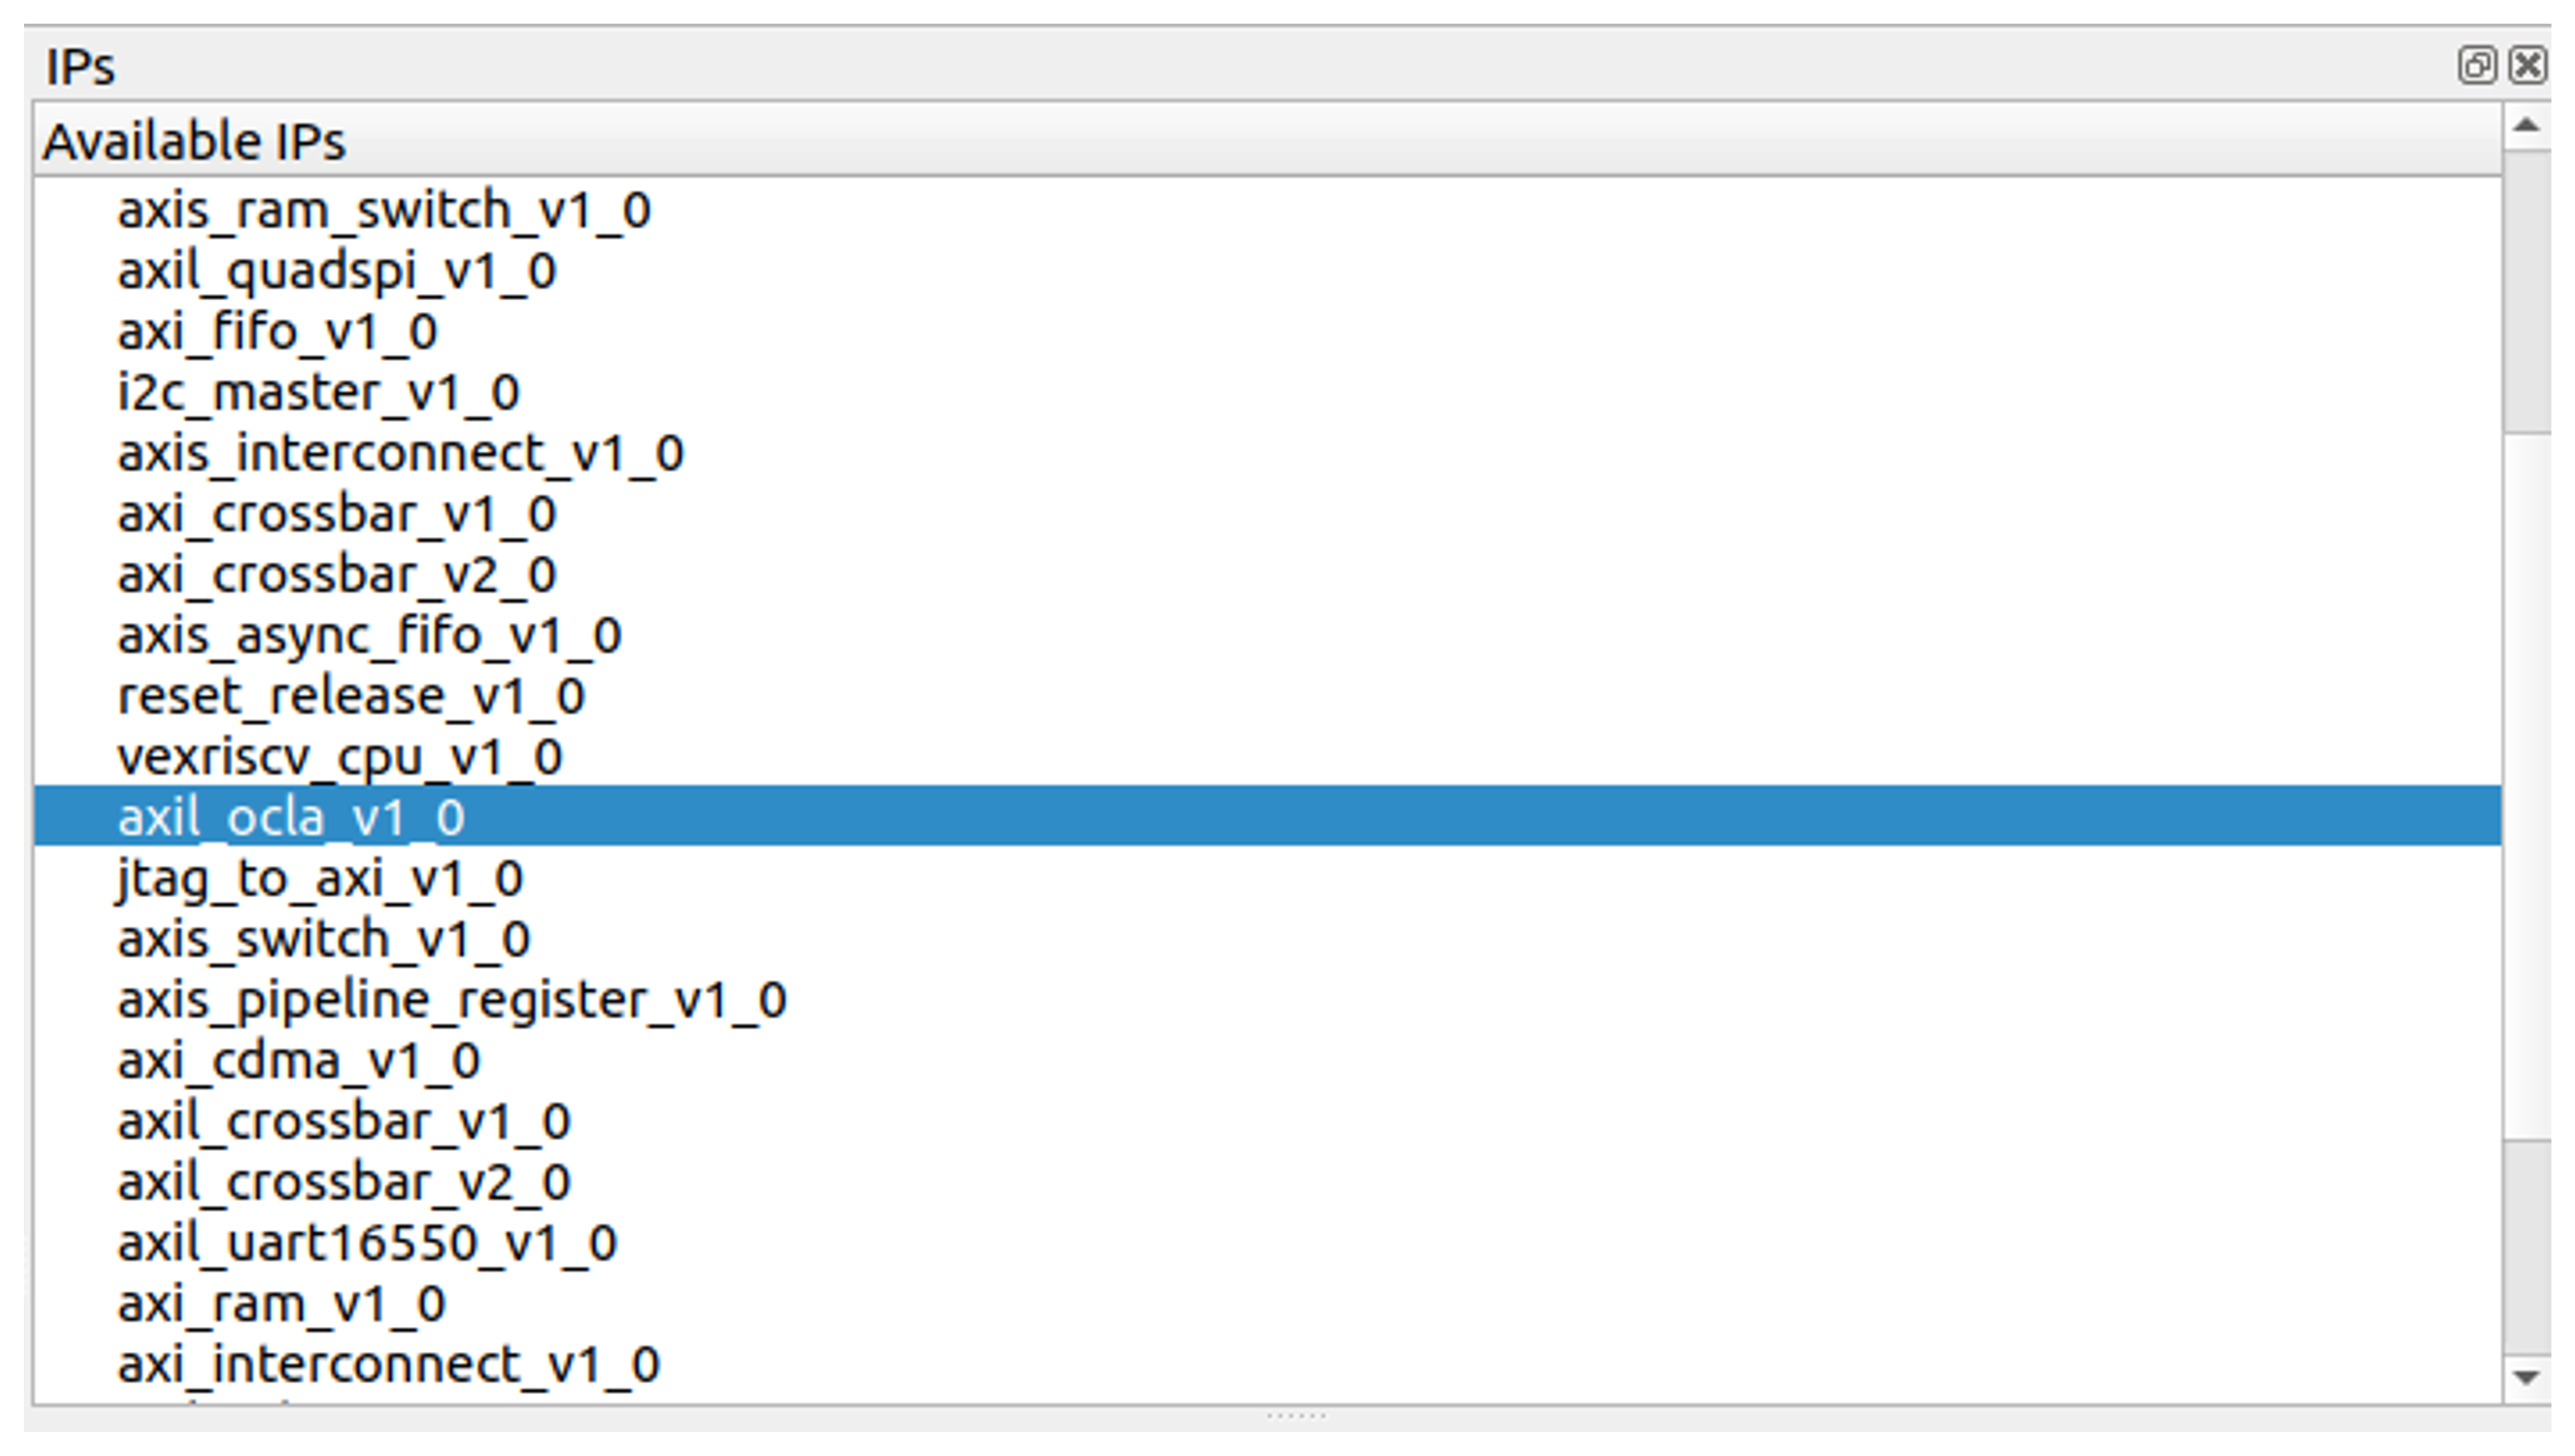
\includegraphics[width=\linewidth]{ip_1}
	\caption{\textbf{Figure \ref{fig:ip_1}.} IP list}
	\label{fig:ip_1}
\end{figure}
% \lipsum
\newpage
\paragraph{Parameters Customization:}
\addcontentsline{toc}{paragraph}{Parameters Customization}
From the IP configuration window, the parameters of the OCLA can be configured and OCLA features can be enabled for generating a customized OCLA IP core that suits the user application requirment.
\begin{figure}[h]\centering % Using \begin{figure*} makes the figure take up the entire width of the page
	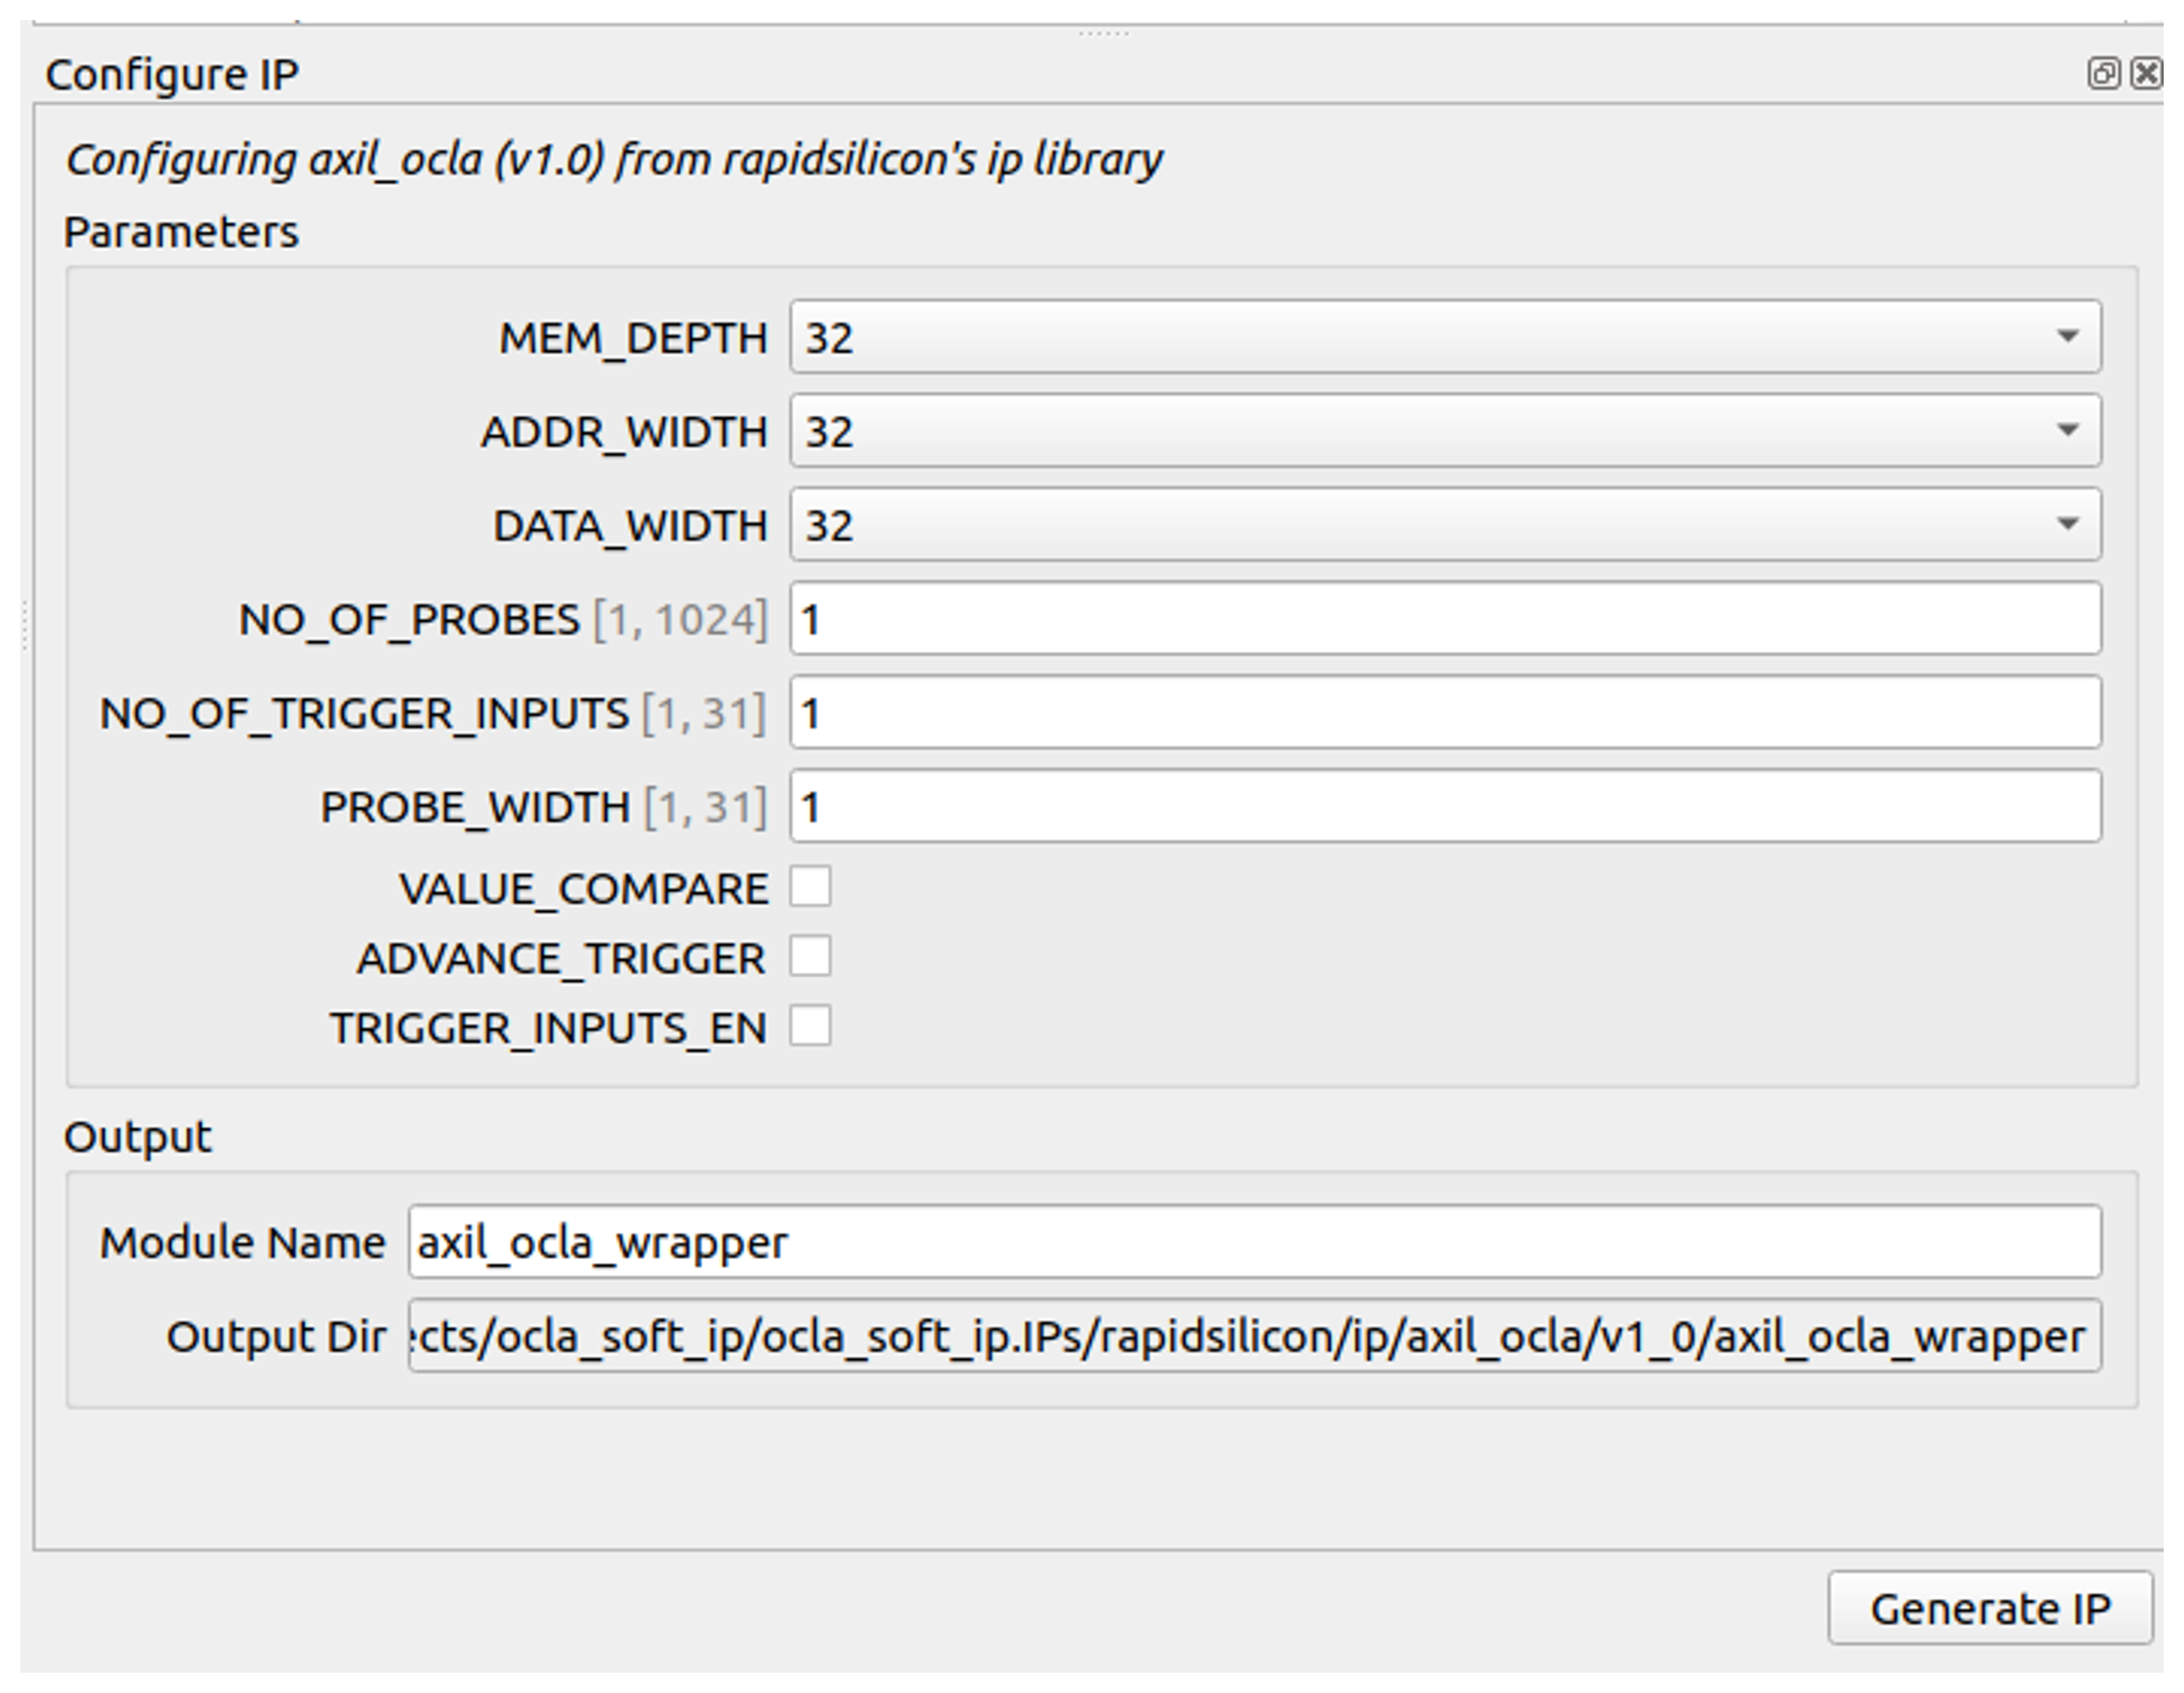
\includegraphics[width=\linewidth]{ip_2}
	\caption{\textbf{Figure \ref{fig:ip_2}.} IP Configuration }
	\label{fig:ip_2}
\end{figure}

% \lipsum


% \lipsum

\newpage

\section*{ \hfill OCLA Debug Subsystem}
\addcontentsline{toc}{section}{OCLA Debug Subsystem}


% \lipsum

\subsection*{\fontsize{14}{16}\selectfont The Generated OCLA IP Wrapper}
\addcontentsline{toc}{subsection}{The Generated OCLA IP Wrapper}

After the IP customization and generation step, a top wrapper plus all source file are made available to the user.\\ 
The generated top wrapper file for OCLA \ref{fig:ocla_wrpr} has two different clocks i.e., the sample clock and the AXI clock. The sample clock of the OCLA is to be connected with
the design being monitored and the AXI clock is to be connected to an AXI bus clock.\\ The signals of the design that are to be sampled are connected to the probes port of the OCLA and the user specified input triggers signals can be connected to the corresponding 
port in the top wrapper. \\For the OCLA configuration and to read the sampled data from the OCLA the AXI-lite slave interface can be connected to an AXI bus.      

\begin{figure}[h]\centering % Using \begin{figure*} makes the figure take up the entire width of the page
	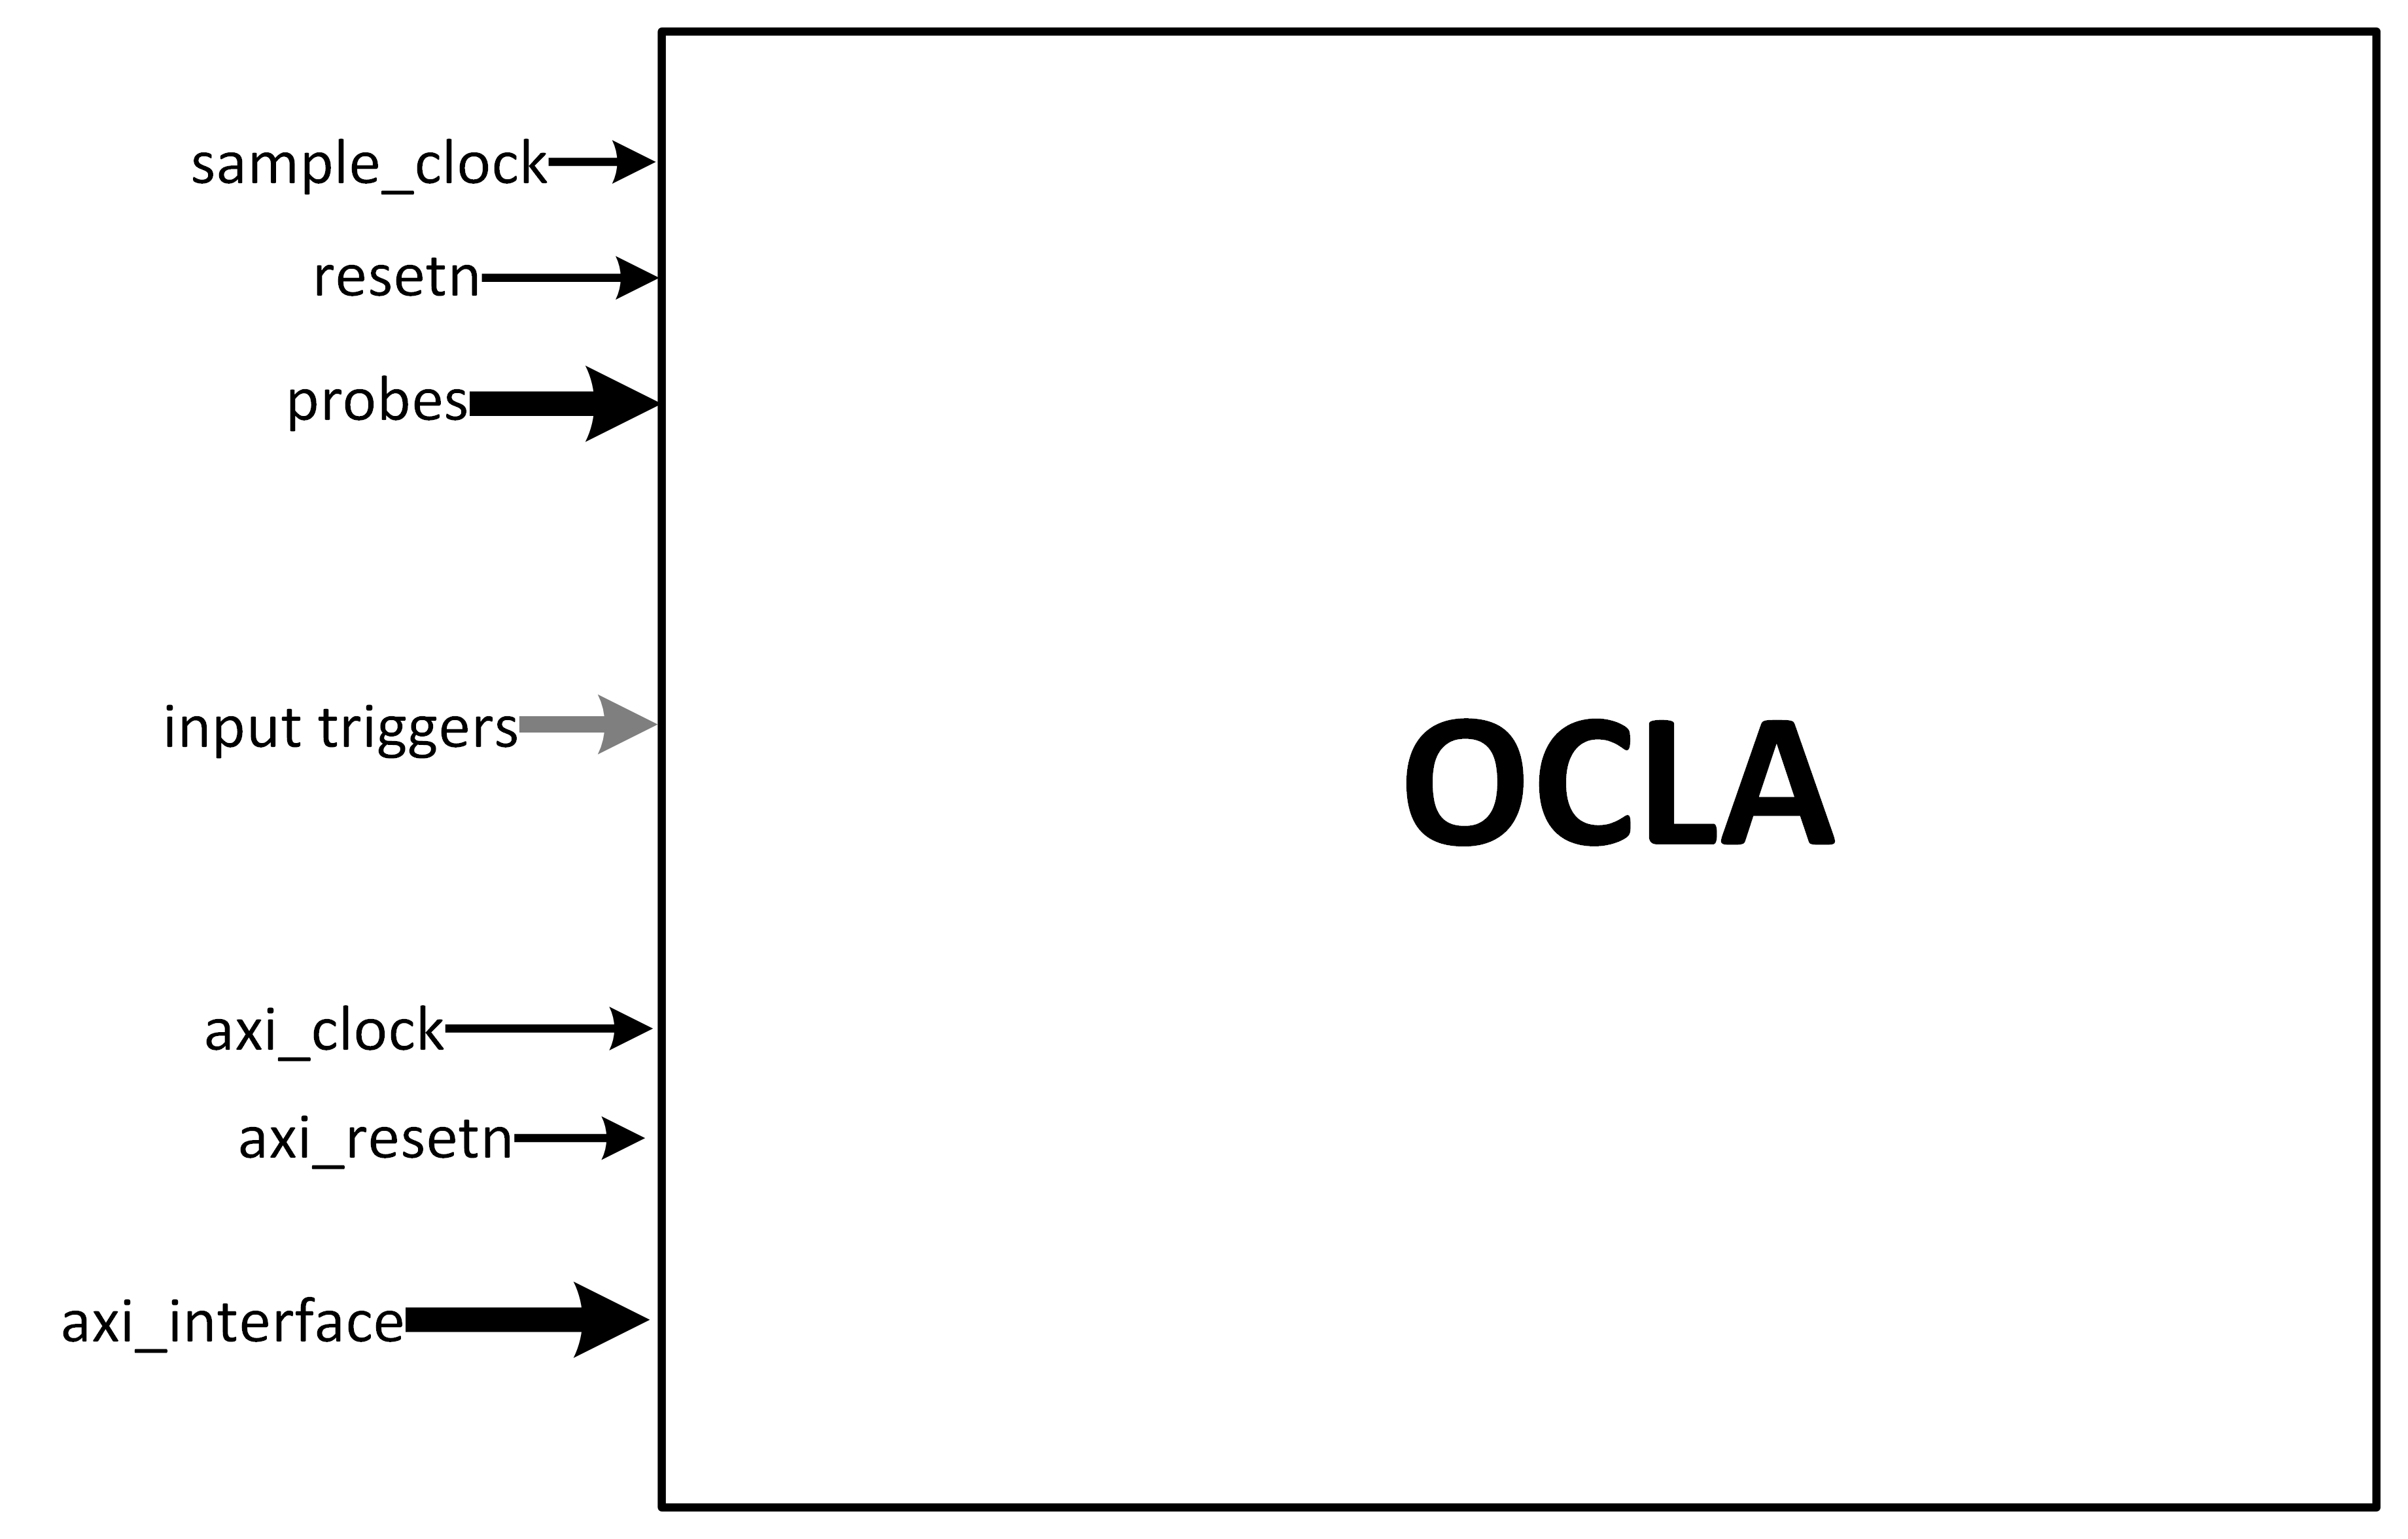
\includegraphics[width=.3\linewidth]{ocla_wrpr}
	\caption{\fontsize{8}{9}\selectfont OCLA TOP}
	\label{fig:ocla_wrpr}
\end{figure}
% \lipsum

\subsection*{\fontsize{14}{16}\selectfont OCLA Debug Subsystem}
\addcontentsline{toc}{subsection}{OCLA Debug Subsystem}
The OCLA top wrapper can be instantiated in a subsystem like the one shown in the figure \ref{fig:ocla_subsystem} for debugging purpose. \\In the debug
subsystem the OLCA IP core is integrated in between the AXI bus and the design being monitored.\\All the runtime OCLA configurations are controlled though JTAG interface.    

% \lipsum

\begin{figure}[h]\centering % Using \begin{figure*} makes the figure take up the entire width of the page
	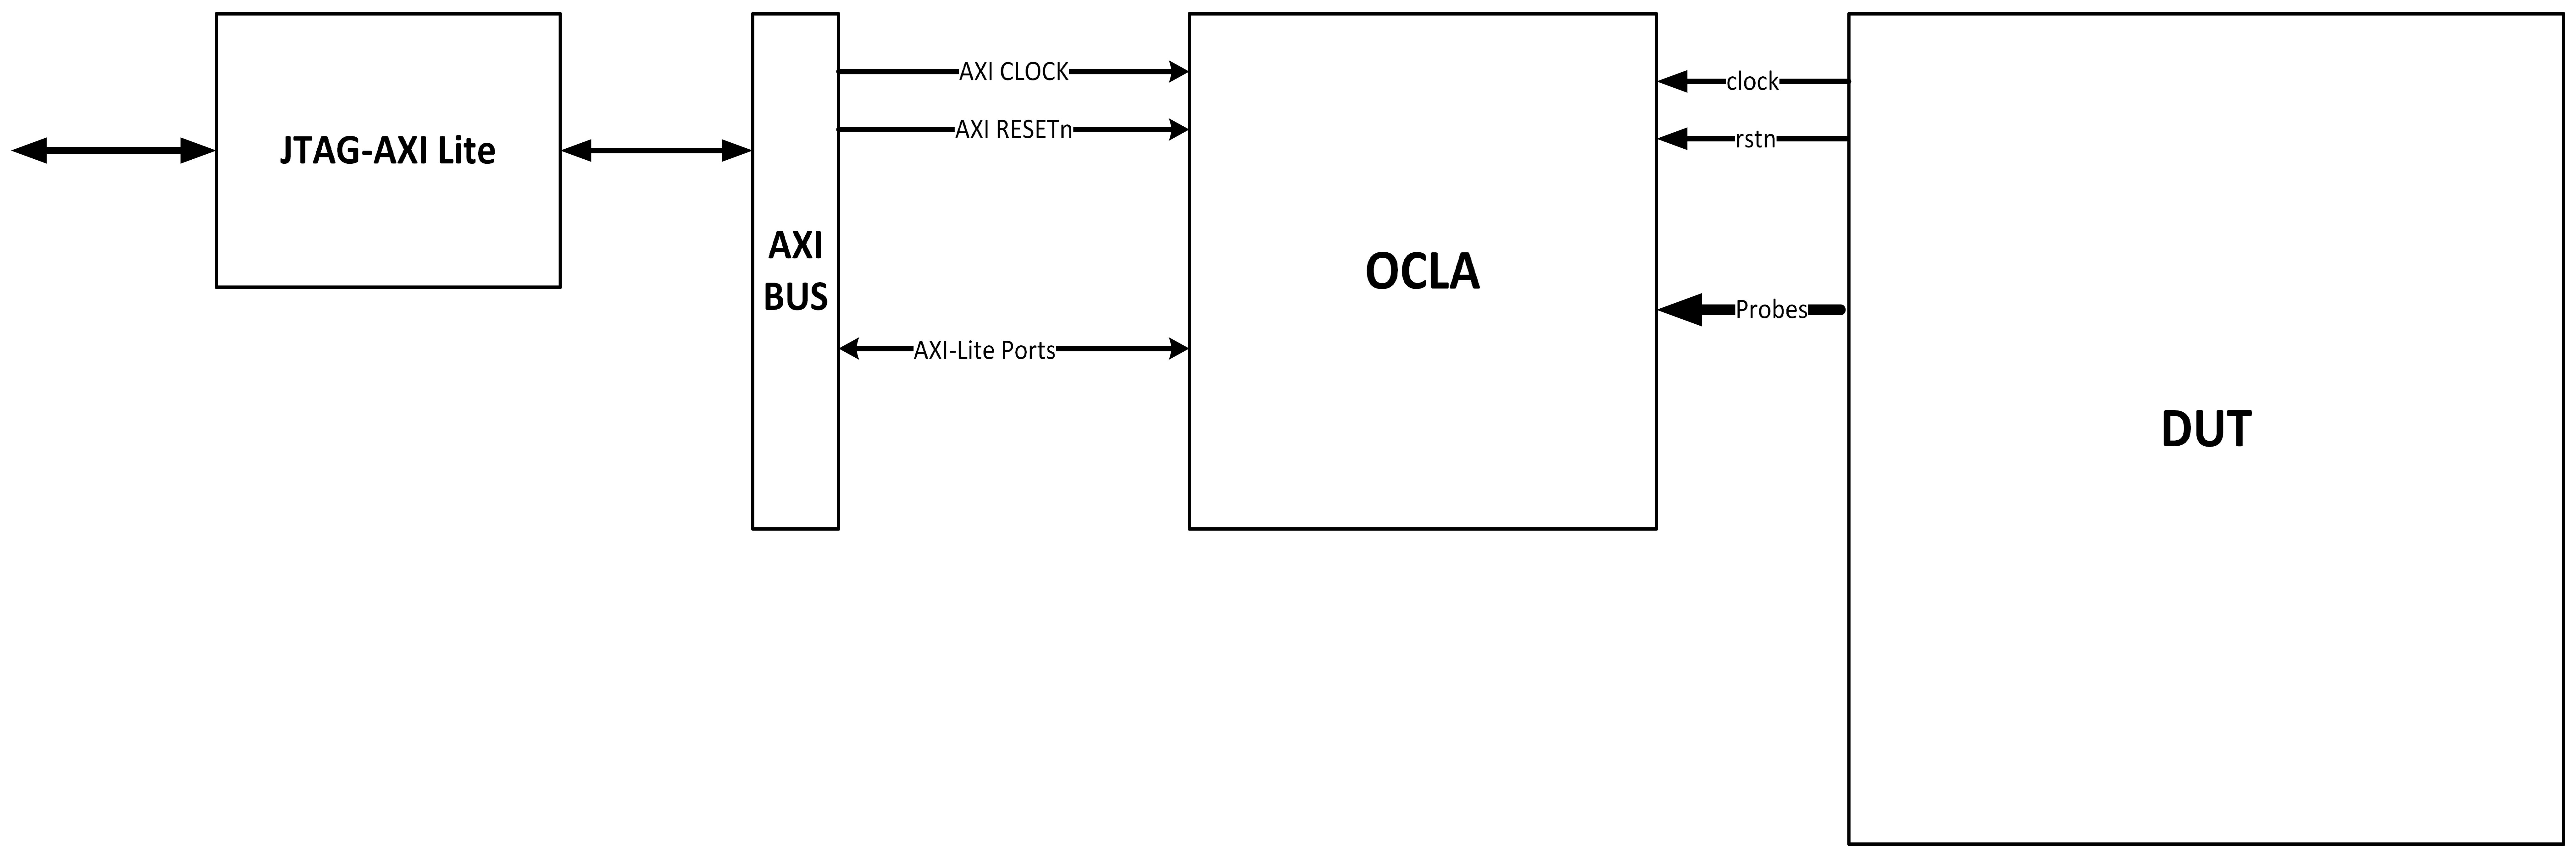
\includegraphics[width=\linewidth]{ocla_subsystem}
	\caption{\fontsize{8}{9}\selectfont OCLA Debug Subsystem}
	\label{fig:ocla_subsystem}
\end{figure}

% \lipsum


% \newpage

\section*{\hfill Example Design}
\addcontentsline{toc}{section}{Example Design}
% \lipsum

\subsection*{\fontsize{14}{16}\selectfont Overview}
\addcontentsline{toc}{subsection}{Overview}

% \lipsum

\subsection*{\fontsize{14}{16}\selectfont Simulating the Example Design}
\addcontentsline{toc}{subsection}{Simulating the Example Design}


% \lipsum

\subsection*{\fontsize{14}{16}\selectfont Synthesis and PnR}
\addcontentsline{toc}{subsection}{Synthesis and PnR}


% \lipsum
\newpage

\section*{ \hfill Test Bench}
\addcontentsline{toc}{section}{Test Bench}

  % \lipsum
  There is no test bench for this IP

% \subsection*{\fontsize{14}{16}\selectfont Testbench Architecture}
% \addcontentsline{toc}{subsection}{Testbench Architecture}

%   % \lipsum


% \subsection*{\fontsize{14}{16}\selectfont Testbench Simulation}
% \addcontentsline{toc}{subsection}{Testbench Simulation}


  % \lipsum



% \usepackage{colortbl}




\raggedright% Right align the text


\newpage
\section*{\hfill  Revision History}
\addcontentsline{toc}{section}{Release} % Adds this section to the table of contents

\addcontentsline{toc}{subsection}{Revision History}




\noindent\begin{minipage}{\linewidth}
	% \centering
	% \captionof{table}{Parameters}\label{tab:param_tab}
	\resizebox{\linewidth}{!}{%
	\begin{tabular}{|l|l|l|} 
	\hline
	\textbf{Date}~                                                               & \textbf{ Version}         & \textbf{ Revisions}                       \\ 
	\hline
	\today & \multicolumn{1}{r|}{0.01} & Initial version OCLA User Guide Document  \\
	\hline
	\end{tabular}
	}
	\end{minipage}

%----------------------------------------------------------------------------------------
}
\end{document}

